\documentclass{llncs}
\usepackage{llncsdoc}
\usepackage{fainekos-macros}

\usepackage[english]{babel}
\usepackage[utf8]{inputenc}
\usepackage{amsmath}
\usepackage{graphicx}
\usepackage[colorinlistoftodos,obeyFinal]{todonotes}
\usepackage{wrapfig}
\usepackage{makeidx}  % allows for indexgeneration
\usepackage{bibspacing}
\usepackage{fancyvrb}
\usepackage{amsfonts}
\usepackage{color}
\usepackage[ruled]{algorithm}
\usepackage{algpseudocode}

\setlength{\bibspacing}{\baselineskip}
\usepackage[tight,footnotesize]{subfigure}

\newcommand{\mySection}[1]{\vspace{-5pt}\section{\hskip -1em.~~#1}\vspace{-10pt}}
\newcommand{\mySubSection}[1]{\vspace{-5pt}\subsection{\hskip -1em.~~#1}\vspace{-10pt}}
\newcommand{\mySubSubSection}[1]{\vspace{-5pt}\subsubsection{\hskip -1em.~~#1}\vspace{-5pt}}
\newcommand{\tableref}[1]{Table~\ref{tab:#1}}
\newcommand{\figref}[1]{Fig.~\ref{fig:#1}}
\newcommand{\Hao}[1]{$\clubsuit$\footnote{HAO: #1}}

\title{Domain-Knowledge-Guided Environment Model Abstraction and Refinement for Medical Device Software Verification}

%\author{You}

%\date{\today}

\begin{document}
\maketitle

\begin{abstract}
This paper proposes a methodology for closed-loop model checking of medical devices, and illustrates it with a case study on implantable cardiac pacemakers.
To evaluate the performance of a medical device on the human body, a model of the device's physiological environment must be developed, and the closed-loop consisting of device (e.g., pacemaker) and environment (e.g., the human heart) is model-checked.
Formal modeling of the environment and its application in model checking pose several challenges that are addressed in this paper.
Pacemakers should guarantee safe operations across large varieties of heart conditions, which are represented by an incomplete set of timed automata models.
A set of domain-specific abstraction rules are developed that can over-approximate the timing behaviors of a heart model or a group of heart models, such that the new behaviors introduced by abstraction are mostly physiologically meaningful.
The rules serve as a systematic method to cover heart conditions that may not be explicitly accounted for in the initial set of heart models.
Closed-loop model checking is systematically performed using the heart models in the abstraction tree, to obtain the most concrete counter-example(s) that correspond to property violation.
These counter-examples, along with their physiological context, are then presented to the physician to determine their physiological validity.
The proposed methodology creates a separation between steps requiring physiological domain expertise (model creation and abstraction rules definition) and steps that can be automated (rule application, model checking, and abstraction refinement).
While the methodology is illustrated for pacemaker verification, it is more broadly applicable to the verification of other medical devices.
\end{abstract}
\section{outline}

\begin{enumerate}
	\item Introduction
	\subitem The problem of closed-loop formal verification
	\subitem In this paper, we illustrate four challenges and solve them for medical devices, specifically cardiac devices. 
	\subitem Some elements of the proposed method can be generalized and have a wider applicability: namely the abstraction tree and MC on the tree (abstractness measure, search procedure)
	\subitem Give overview of method in a block diagram and briefly explain it in text.
	
	\item Formal models of the environment
	\begin{enumerate}
		\item Heart basics, enough to understand the proposed models
		\item Emphasis: different heart conditions necessitate different models.
		\item Creation of formal heart models: graph structure + node and path automata
		\item Two examples of heart conditions and their formal models.
		\item Emphasis: our initial set of models is not necessarily complete. That is, there are more heart conditions that could be modeled, but aren't. It is always a work in progress.	
		\subitem Therefore we want to add behavior to try and cover things not covered by the models. Adding models i not the answer since it will always be an incomplete set. Not to mention it's a manual process.
		\item Formalization of physiological requirements
	\end{enumerate}
	
	\item Abstraction rules: how to add behavior to the initial set of models
	\begin{enumerate}
		\item Why predicate-based abstraction can be inadequate?
		\label{ar:inadequate}
		\subitem If we get a cex which is spurious by the classical definition, it is not necessarily spurious physiologically. Remember we are enriching the behavior precisely to cover new conditions.
		\subitem So it's up to the physician to decide if the cex is spurious or not. But predicate-based abstraction might give hard-to-understand cex.
%		\subsubitem Two ambiguities: interaction and context ambiguities. Interaction ambiguity because the requirement is purely on the env.
		\subitem Example
		\subitem Therefore, need the added behavior to be physiologically meaningful so it's understandable.
		\item Physiologically meaningful abstraction rules
		\subitem Give formal definition of a rule as a graph-to-graph function $R: G \rightarrow G'$ 
		\subitem Why do you call it abstraction? 
		\subitem Given 2 concrete examples (more in tech report)
		\item Example of rule application.
		\item Abstraction tree		
	\end{enumerate}
	
	\item Model-checking with the abstraction tree
	\begin{enumerate}
		\item Measure of abstractness; define 'appropriate for the requirement'
		\item Search procedure
		\item What happens if a counter-example is found: give the physician the most concrete model on which the cex still shows up.
		\item Case study: i.e., elaborate example
	\end{enumerate}
	
	\item Conclusions and future research
	
\end{enumerate}



\section{Introduction}
\label{introduction}

Implantable medical devices like pacemakers are designed to improve physiological conditions with very little human intervention. 
Their ability of autonomously affecting the physiological state of the patient makes the medical devices safety-critical, and sufficient evidence for their safety and efficacy should be provided before the devices can be implanted in the patients. 
As more functionality is added to the devices
\footnote{In what follows, we use the word `device' to refer both to the hardware and the software of the device.}
, the complexity of the software component of the device is increasing dramatically, leading to a large number of potential safety violations due to software bugs \cite{recall_stats}.


There are two categories of device bugs: 
1) the device may fail to conform to its \emph{specifications}, i.e. the prescription of how it should react to certain inputs.  
2) the device may fail to improve the conditions of the patient as promised, even if it conforms to its specifications. 
The desired physiological conditions that the closed-loop system should achieve are captured in the \emph{physiological requirements}; e.g., for a pacemaker, the heart rate should always be maintained above a certain threshold. 
%In what follows, the word `requirement' always refers to such physiological requirements.
%Note that requirements are about \emph{the closed-loop system}: they prescribe the behavior of both device and environment (e.g. both pacemaker and heart).

Bugs in the first category (non-conformance to specification) can be detected via systematic and extensive open-loop testing in which a set of input sequences is fed to the device, and its output is compared with the expected output.
Bugs in the second category (violation of physiological requirements), on the other hand, require the availability of the \emph{closed-loop system}, which consists of the device and its environment.
E.g., the pacemaker and the heart as its environment. 
In the medical device industry, closed-loop verification of the physiological requirements are mostly performed in terms of clinical trials, in which the actual devices are implanted in human subjects over an extended duration.
Unfortunately, due to the extremely high cost, the amount and variety of human subjects during the clinical trials are limited, which reduces the number of bugs found during trials. 
\todo{give dollar amount}
Moreover, clinical trials are often conducted at the last design stage. Fixing bugs at this stage is very costly.

Closed-loop model checking enables closed-loop evaluation of the physiological requirements at an earlier design stage, which requires formal model(s) of the physiological environment. 
%Depending on the formalism used to model the environment (and device) and the language used to express the requirements, this allows the usage of formal methods to perform the verification.
%Formal environment modeling introduces new challenges that do not arise when modeling the device alone, and this paper aims at addressing these issues in the context of pacemaker verification.
%In the rest of this paper, we speak therefore of pacemaker as the Device Under Verification (DUV) and of the heart as being the environment, but it is understood that the discussion carries more broadly, with possible domain-specific adjustments.
In closed-loop model checking, there is only one concrete system. However there can be countless number of environmental conditions which require different models to represent. A set of initial models of the environment can be constructed but the set is inherently incomplete due to the large number of environment conditions and their combinations. As the result, performing model checking using every models in the set cannot ensure full coverage on environment conditions. 

Over-approximation has been proposed in system modeling to reduce the state space while covering all the behaviors of the system. Over-approximation can be extended to environment modeling. By carefully designing over-approximation rules, the abstract model not only covers explicitly modeled environment conditions, but also covers behaviors and conditions not modeled in the set of initial models. The abstract model can be then used for closed-loop model checking. If a requirement is satisfied, the system under verification satisfy the requirement under environment conditions covered by the abstract model. 

However, if the requirement is unsatisfied, the model checker returns a counter-example. The counter-example is not necessarily a bug since it may be a behavior that does not belong to any environment conditions, but was introduced into the abstract model during over-approximation. In system modeling the validity of the counter-example can be easily checked on the one and only concrete system. However in environment modeling, due to the possibly valid behaviors introduced in the abstract model, the validity of the counter-example cannot be determined even if it is not valid in all the models in the initial model set. Thus the validity of a counter-example can only be determined by domain experts, which is made challenging due to the possible lose of environment context during the over-approximation. One abstract counter-example may also correspond to multiple valid conditions, which causes ambiguity. A rigorous framework is thus needed to balance the coverage and environment context of the environment models.

Counter-Example Guided Abstraction and Refinement (CEGAR) \cite{CEGAR} has been proposed to over-approximate the system using predicate abstraction. Upon property violation the abstract counter-example is checked for its validity on the actual system. If the counter-example is \emph{spurious} the model is then refined to eliminate the spurious counter-example. This process is then continued on the refined model until either a valid counter-example returns or no counter-examples are returned. CEGAR works well during system modeling, however, it cannot be applied to environment modeling for two reasons: 1) predicate abstraction does not guarantee the validity of behaviors introduced into the model. In fact, for system modeling, all additional behaviors introduced into the abstract model are spurious. 2) the validity of a counter-example cannot be checked automatically as in system modeling.

Another challenge for closed-loop model checking of medical devices is the amount of domain expertise needed during: 1) Physiological modeling; 2) Physiological model abstraction and refinement; 3) Checking the validity of counter-examples. In \cite{sttt13} we developed a set of heart models with different abstraction levels for closed-loop model checking of implantable pacemaker. In each steps of closed-loop model checking, both physiological knowledge and knowledge on formal methods are needed, which is not idea in real world applications. %The models were constructed and abstracted manually using domain knowledge. Models at different abstraction levels have a timed simulation relationship which are also proved manually. Upon property violation in an abstract model, the validity of the counter-example is checked manually and the appropriate refinement is also chosen manually to eliminate spurious counter-examples. 

\subsection{Contributions}
In this paper we propose a framework for environment modeling in closed-loop model checking of medical device software, which separates physiological knowledge and formal method knowledge required during each model checking steps. We use implantable pacemaker and heart modeling as an example. An expandable set of heart models are first developed to represent different physiological conditions. A set of physiological abstraction rules are then developed based on physiological knowledge, which ensure the physiological relevance of the behaviors introduced into the abstract models. Then the rules are applied to the initial set of physiological models to obtain an abstraction tree, which will be used for closed-loop model checking of pacemaker. A simple search procedure is then used to conduct model checking using suitable heart models and return the most concrete an unambiguous counter-examples to the physicians for analysis. In this framework, physiological knowledge is only needed when constructing the initial model set and analyzing counter-examples. The application of physiological abstraction rules and performing model checking can be automated.

%During the closed-loop model checking, the most abstract model(s) that are appropriate to the requirement are automatically selected as the initial environment models. If the requirement is satisfied, the system is safe under the environment conditions covered by the initial environment models. If the requirement is violated in certain initial environment model, the children of the model in the abstraction tree are used for model checking until 1) the leaves of the tree is reached, or 2) there is no violations in the child nodes. The counter-examples obtained at the most refined models are returned to the physician for validity check. This process is automated so that no domain knowledge is required for the person who performs model checking. It also ensures the most concrete counter-examples with unambiguous physiological context are returned to the physician for analysis. 
%The first challenge in closed-loop model checking of pacemakers is that the human heart displays a large number of different conditions, henceforth referred to as `physiological conditions'.
%E.g., one heart may display \emph{atrial fibrillation} where the upper chambers of the heart (the atria) produce an exceedingly fast beat that prevents proper blood pumping.
%Another heart may display Premature Ventricular Contraction (PVC) where a location in the ventricles produces electrical impulses at erratic time instants.\Hao{I don't think these two conditions make sense to the reader}
%Each such condition will require its own formal model, and some models may display more than one condition.
%In this paper, we build such a set of formal heart models using the timed automata formalism in Section ???.
%Performing model checking with each model separately, we seek a method that can combine models, and perform model checking on the merged model. 
%The combination of models must be such that if the merged model is correct (according to the requirements) then so is every model that was combined into it.
%We present \emph{abstraction rules} in Section ?? which allow us to do precisely that.

%This initial set of models will necessarily be \emph{incomplete} because the number of physiological conditions is too large, and some of the conditions are too ill-understood for modeling.
%Thus, unlike system modeling in which one typically starts from one ground truth model to be verified, our starting point is an \emph{incomplete set of environment models}.
%Because of this incompleteness, we seek abstraction rules that introduce new \emph{physiologically meaningful} behavior which might actually be produced by heart models not in the initial set.
%These then correspond to heart conditions not taken explicitly into account. 
%This provides a second motivation for the domain-specific abstraction rules $R$ in Section ???, which can be thought of as relaxations of the conditions governing the model's behavior. 
%Like predicate abstraction, they produce models that over-approximate the behavior of the model they are applied to (i.e., $\beh(R(M)) \supset \beh(M)$).
%However, the new behavior they introduce might not be spurious. 
%We demonstrate such a case in Section ???.
%If model checking returns a counter-example on $R(M)$, the physician can decide whether this is actually physiologically plausible behavior and therefore the pacemaker needs to be debugged, or this is indeed spurious and should be thrown out (and the abstraction refined).
%
%Note this is different from classical predicate abstraction [???], which adds behavior in a domain-agnostic fashion. In fact, predicate abstraction is a fist step in the timed automata model checking procedure as presented in [ALur and Dill 1994].
%Our abstraction rules are used to combine and and abstract models \emph{prior} to model checking.
%%tttt
%
%\subsubsection{Contributions}
%In this paper we propose a framework for environment modeling and model checking of medical device software, in particular, pacemakers.
%Specifically, we present several extended timed automata models of various heart conditions in Section ???. 
%We define domain-specific abstraction rules for these models, and demonstrate how these can be applied to gradually add physiologically meaningful behavior in Section ???. 
%Using the models and the rules, we build an abstraction tree which serves to perform model checking of physiological requirements for the heart+pacemaker closed loop in Section ???.
%We illustrate the approach via case studies in Section ???, and conclude in Section ???
%
The proposed method can potentially generalized to other domains in which the system operates in a large variety of environmental conditions.
%

%\section{Formal Models of the Environment}
\label{formalModelsofEnv}
To perform closed-loop model checking of medical devices, formal models of their physiological environment are needed to represent different physiological conditions the devices may encounter. In this section, implantable pacemakers are used as example. Timed-automata \cite{timed_automata} models of the human heart are developed as the environment model \cite{sttt13,VHM_proc}. Physiological requirements are formalized with monitors and $ATCTL^*$ formula \cite{TCTL}. 
Model checking can then be performed on the closed-loop system with UPPAAL \cite{uppaal}. %The physiological knowledge required during closed-loop model checking of medical devices are associated with the \emph{physiological models} and the \emph{physiological requirements}. It is thus important to maintain the physiological context of the models and link model behaviors to physiological requirements. In this section we use heart modeling as example to demonstrate physiological knowledge encoding. %First, we introduce the physiological basis for our heart modeling. Then we demonstrate our heart model structure which can be used to model different heart conditions. We link transitions in the models to physiological behaviors
\begin{figure}[!t]
	\centering
	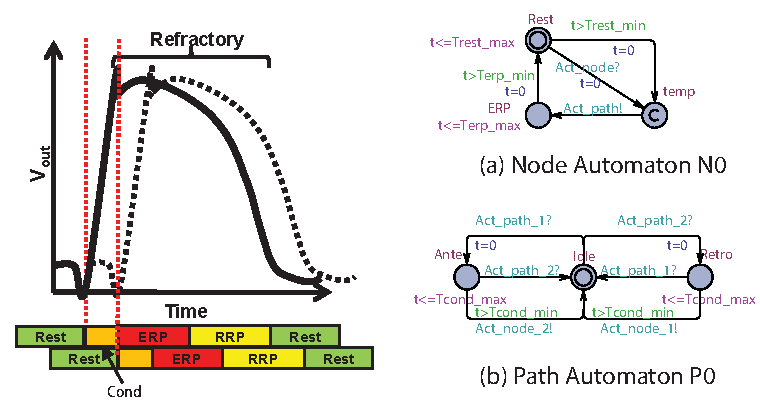
\includegraphics[width=0.9\textwidth]{figs/init_abs.pdf}
	\vspace{-10pt}
	\caption{\small (a) Action potential for a heart tissue and its tissue nearby (dashed). (b) Node automaton. (c) Path automaton. (d) An example model of the heart consist of a network of node and path automata. The nodes are labeled with the name of the corresponding physiological structures.}
	\vspace{-15pt}
	\label{fig:nodepathTA}
\end{figure}

\subsection{Timed-automata Models of the Heart}
At cellular level, a heart tissue can be activated by external voltage. Certain tissue also has capability to self-activate, which contribute to natural heart beats. Once activated (Marker 1 in \figref{nodepathTA}), the voltage outside the tissue changes over time, which is referred to as \emph{Action Potential} (\figref{nodepathTA}.(a)). 
The action potential can be divided into two functional timing periods: The \emph{Effective Refractory Period (ERP)}, during which the tissue cannot be triggered by another activation; and the \emph{Rest} period, during which the tissue can be activated and at the end of which the tissue will self-activate. 
The timing behaviors of the action potential are modeled as \emph{node automaton} $A_v$ (\figref{nodepathTA}.(b)). 
A node automaton initializes with \textsf{Rest} state.
From \textsf{Rest} state, the node can either self-activate or be activated by external activations (indicated by Act\_node). 
Upon activation the node transition to the \textsf{ERP} state and activate all the paths connecting to the node (indicated by Act\_path). 
In the \textsf{ERP} state the node does not respond to external activations. 
At the end of \textsf{ERP} state the node transition to the \textsf{Rest} state. 
The duration a node automaton can stay in \textsf{Rest} is in the range $[Trest\_min,Trest\_max]$, and the duration it can stay in \textsf{ERP} is in the range $[Terp\_min, Terp\_max]$.
For heart tissue without the capability to self-activate, the parameters $Trest\_min$ and $Trest\_max$ are set to $\infty$.
$Trest$ and $Terp$ are referred to as \emph{parameters} of the automaton $A_v$.

The voltage change of the heart tissue will activate the tissue nearby with certain delay (Marker 2 in \figref{nodepathTA}). 
This timing delay between heart tissue is modeled using \emph{path automata} $A_e$ (\figref{nodepathTA}.(c)). 
The initial state of a path automaton is \textsf{Idle}, which corresponds to no conduction. 
A path has two conduction directions, forward and backward.
These are represented by the states \textsf{Ante} and \textsf{Retro}, named after their standard physiological terms Antegrade and Retrograde.
If \textsf{Act\_path} event is received from one of the nodes (1 or 2) connected to the path, the transition to \textsf{Ante} or \textsf{Retro} state will occur in the path automaton. 
At the end of \textsf{Ante} and \textsf{Retro} state the path will transition to \textsf{Idle} state and send Act\_node signal to the node automaton connected to the other end of the path (2 or 1).
The parameters of the path automaton $A_e$ are $Tcond$.

A healthy heart generates periodic electrical impulses to control heart rates according to physiological needs. 
These impulses propagate through the heart, triggering coordinated muscle contractions and pump blood to the rest of the body. 
The underlying pattern and timing of these impulses determine the heart's rhythm and are the key to proper heart functions. 
Derangements in this rhythm are referred to as \emph{arrhythmia}, which impair the heart's ability to pump blood and compromise the patients' health. 
Arrhythmias are categorized into so-called Tachycardia and Bradycardia. 
Tachycardia features undesirable fast heart rate which results in inefficient blood pumping. Bradycardia features slow heart rate which results in insufficient blood supply. Different heart conditions can be distinguished by the \emph{timing} of the electrical conduction, and the \emph{topology} of the electrical conduction system of the heart, which are researched in clinical setting referred to as \emph{Electrophysiology (EP)}\cite{josephson}. 
%Heart tissue can be modeled as \emph{Node automata} and the conduction delays between nodes are modeled as \emph{Path automata} (\figref{nodepathTA}). 
%\hatodoin{Last sentence repetitive?}


%\subsection{Timed-automata Models of the Heart}
%\label{labeledGraph}
%In a healthy heart, specialized tissue in the \emph{SA node} self-activate periodically. The signal conducts throughout both atria, causing them to contract and push the blood into the ventricles
%Models of different physiological conditions have to be developed to be able to interact with the medical devices. This initial set of physiological models should be able to distinguish the physiological conditions that each model represents. Ideally the models are developed using formalisms that are suitable for provable abstraction and model checking. 

%A node automaton models the conduction states of heart tissue, and changes therein. 
%Its three states correspond to 3 timing periods of the action potential. 
%From \textsf{Rest} state, the node can either self-activate or be activated by external stimuli (both events are indicated by Act\_node) and transition to the \textsf{ERP} state. 
%In the \textsf{ERP} state the node does not respond to external stimuli because it is refractory. 
%In the \textsf{RRP} state, the node can still be activated and transition to the \textsf{ERP} state.
%But the fact that the activation arrived early (in the RR Period) affects the ERP and the conduction delay of the tissue.  
%%This is tracked by a shared variable $C(i)$ for the $i^{th}$ node automaton. \todo[inline]{what is $C$?}
%%The new ERP period is determined by a function over clock value $g(f(t))$ which mimics the beat-to-beat dynamics described in \cite{josephson}. \todo[inline]{what are $g,f$?}
%
%The electrical conduction through the tissue \emph{between} nodes is abstracted using \emph{path automata}. 
%The path automata are used to represent structural or functional electrical connections between nodes. 
 \begin{figure}[!t]
	\centering
	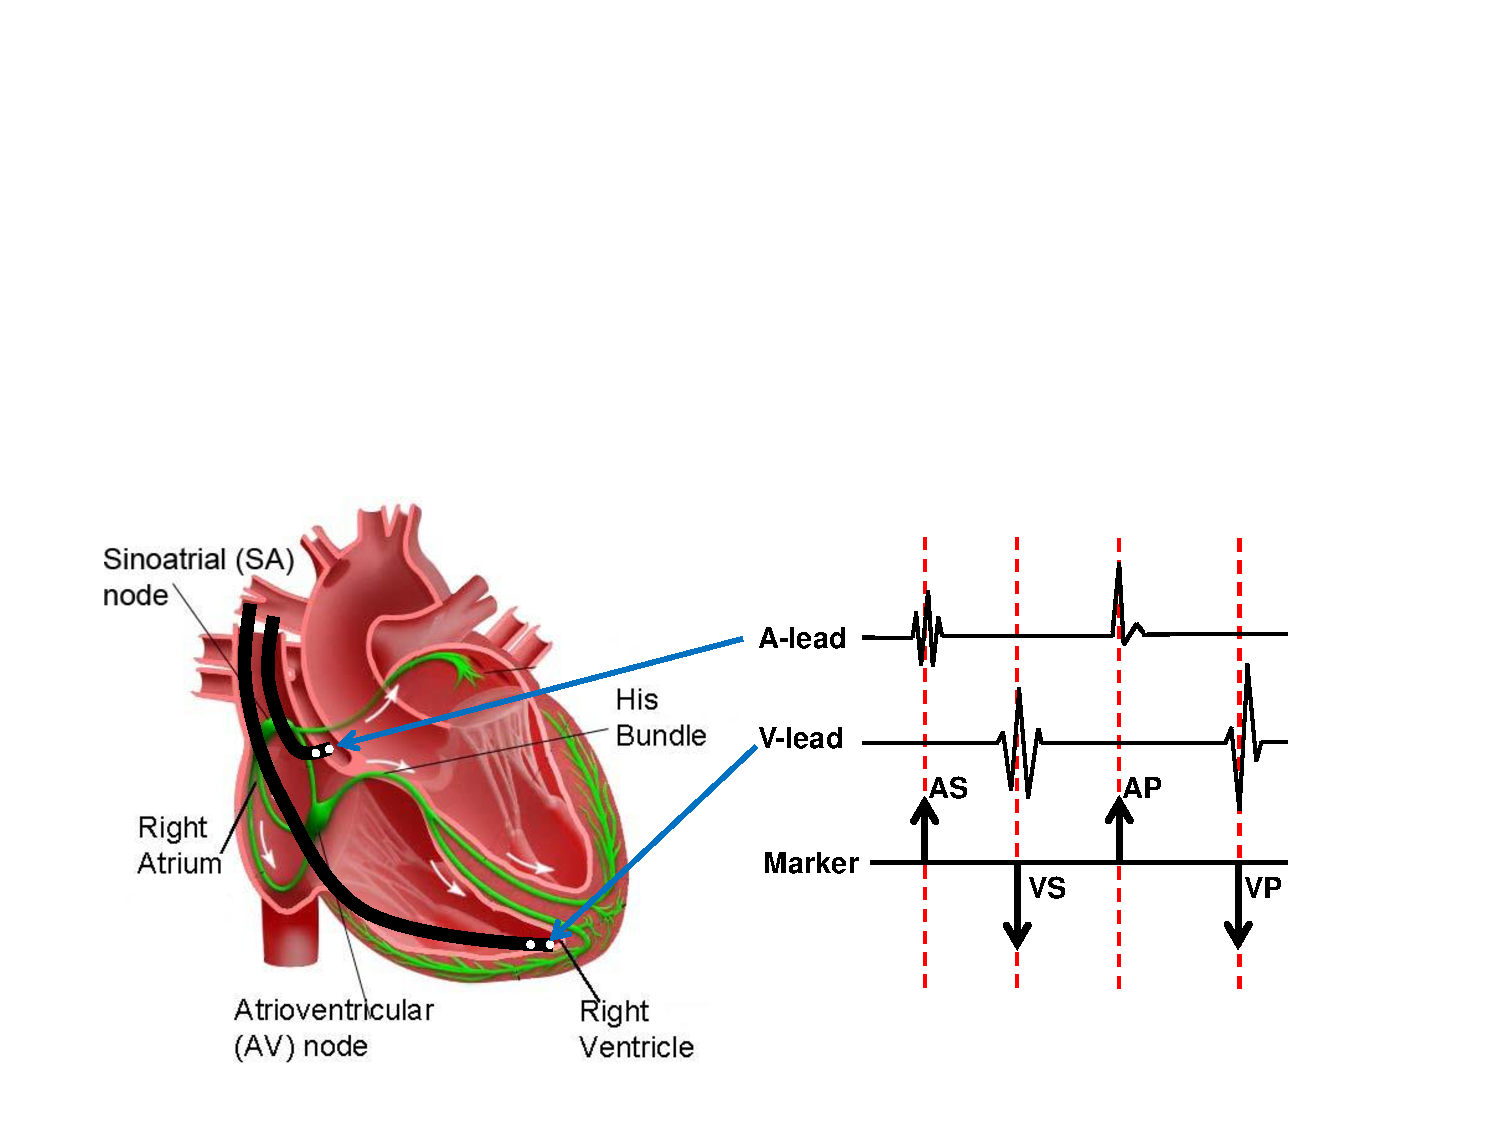
\includegraphics[width=0.7\textwidth]{figs/egm.pdf}
	
	%\vspace{-10pt}
	\caption{\small (a) Lead placement for a dual chamber pacemaker (b) Electrogram (EGM) signals from pacemaker leads and corresponding internal event markers}
	\label{fig:probes}
	\vspace{-10pt}
\end{figure} 
%%At the same time the clock invariant of the state is modified according to the shared variable $C(a/b)$. 
%%This corresponds to the change of the conduction delay that is caused by early activation. 
%Similarly to a node automaton, the changing trend is extracted from clinical data. 
%
%The parameters of the node and path automata determine the ranges of time in which the automata can stay in corresponding locations. 
%The lower endpoint is specified as a clock invariant and the upper endpoint is specified as a guard. 
%For a heart model $G$ with $n$ nodes and $m$ paths (thus, $n$ vertices and $m$ edges), the node automata are denoted as $N_i, i\in[n]$ and path automata are denoted as $P_j,j\in[m]$. 
%\todo[inline]{change to $V_i$ and $E_i$ to stay consistent with definition of graph?}
%The parameters for the nodes are $Trest$ (with range $[Trest_{min}$),TERP,TRRP and the parameters for the paths are $\{Tante,Tretro\}$. 
The spatial and temporal properties of a given human heart condition can be modeled by a network of node and path automata with different parameters (i.e., \figref{nodepathTA}.(d)). Physiological structures of the heart are represented as node automata and the path automata specify the connectivities of the nodes and the conduction delays among them. 
The network can be viewed as a labeled directed graph: %the vertices of the graph represent nodes, or locations, in the heart, while edges represent conduction paths between the nodes. 
\begin{defn}
	\label{def:labeledGraph}
	[Labeled graph]
	A \textbf{labeled graph} is a directed graph $G = (V,E,A)$ where 
	$V$ is a finite set of vertices, $E \subset V\times V$ is a finite set of directed edges,
	and $A$ is a total labeling function $A: V \cup E \rightarrow TA$
	where $TA$ is the set of timed automata.
	The function $A$ labels each vertex with a \emph{node automaton}, and each edge with an \emph{path automaton}.
	For a graph $G$, we write $\Ec(G) \defeq V(G) \cup E(G)$.
\end{defn}
The heart model structure has been used to model various heart conditions and all of them have been validated by electrophysiologists \cite{vhm_ecrts10,vhm_embc10}.

Implantable cardiac pacemakers are rhythm management devices designed to treat bradycardia. 
A typical dual chamber pacemaker has two leads inserted into the heart through the veins which can measure the local electrical activities of the right atrium and right ventricle, respectively. According to the timing between sensed impulses the pacemaker can deliver electrical pacing to the corresponding chamber to maintain proper heart rhythm (\figref{probes}).  



%\subsection{Describe Model Behaviors with Physiological Context}
%During model abstractions, the abstract model covers all transitions of the more refined model. Transitions corresponding to physiological behaviors may be merged or replaced by other transitions. Without documenting these information, the abstract models lose their physiological context. 
%In the heart models we modeled physiological timing periods using locations in timed automata. The minimum time an automaton can stay in those locations is limited by the guard on a transition out of the location, and the maximum time is limited by the clock invariant of the state. 
%The transitions of heart tissue can be categorized into 3 basic transition groups:
%\begin{itemize}
%	\item \textbf{self:} The self-activation of the node automata. The \emph{min} and \emph{max} parameters equal to $Trest\_min$ and $Trest\_max$ parameters in the node automata, which specify the minimum and maximum intervals between consecutive self-activation events.
%
%	\item \textbf{block:} The blocking property of the node automata. The \emph{min} and \emph{max} parameters equal to $Terp\_min$ and $Terp\_max$ parameters in the node automata, which specify the minimum and maximum intervals between consecutive activations that can trigger path conduction.	
%	\item \textbf{cond:} The conduction property of the path automata. The \emph{min} and \emph{max} parameters equal to $Tcond\_min$ and $Tcond\_max$ parameters in the node automata, which specify the minimum and maximum delays between a node activation on one end and the activation on the other end.
%\end{itemize}
%As an example, a node automata $NA$ has two transition groups, which can be represented by $NA.self$ and $NA.block$
\begin{figure}[!t]
		\centering
		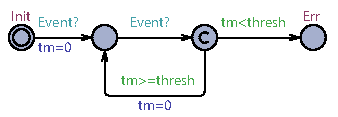
\includegraphics[width=0.8\textwidth]{figs/monitor.pdf}
		%\vspace{-5pt}
		\caption{\small (a) $M_{sing}$ for single event; (b) $M_{doub}$ for two events}
		  \vspace{-10pt}
		\label{fig:monitor}
\end{figure}
\subsection{Formalizing Physiological Requirements}
%Devices are designed to improve certain physiological conditions, the performance of the devices is evaluated on the difference between the patient conditions without the device and with the device. The device should also avoid deteriorating certain patient conditions, physiological requirements are specified in the form of:
%$$C_{pre}\rightarrow C_{post}$$
%in which $C_{pre}$ is the physiological conditions without the device,  and $C_{post}$ is the physiological condition with the device. For model-based closed-loop verification, $C_{pre}$ is often in form of a set of constraints on patient parameters. As a special case, $C_{pre}$ can equal to $true$, means that $C_{post}$ should be satisfied under all possible conditions.
%
%Physiological requirements are constraints on physiological behaviors. In \cite{iccps10} we 
%
%\subsection{Monitors}
Physiological requirements must be formalized for closed-loop model checking. In the case of medical devices, the devices are designed to \emph{improve} certain physiological conditions. 
%For an unhealthy open-loop physiological condition that a device is designed to improve, the closed-loop condition should be healthy.
Software developers are particularly interested in the scenario in which a healthy open-loop physiological condition became an unhealthy closed-loop condition due to device intervention, which is a bug in the device.

In general, a closed-loop requirement $\varphi$ is in the form of $\varphi_E\Rightarrow \varphi_C$, in which $\varphi_E$ is the open-loop physiological condition that the device encounters, often in form of parameter ranges in the environment models, and $\varphi_C$ is the closed-loop physiological condition that the device should achieve. Then we have:
\begin{equation}\label{req_def}
M_E\models\varphi_E \land M_E||M_D\models \varphi_C\Rightarrow M_E||M_D\models\varphi
\end{equation}
%\hatodoin{What is this comma in the equation? is is AND, or OR, or something else?}
%A requirement $\varphi: \varphi_E\Rightarrow \varphi_C$ contains open-loop environmental constraints in $\varphi_E$ and desired closed-loop condition specified in $\varphi_C$.  
The substates for a heart model are clocks and locations for each node and path automata. In \cite{vhm_iccps11}, physiological heart conditions are mapped to constraints on substate variables of the heart models, which can be written as atomic propositions. General monitors are also developed in Stateflow \cite{stateflow} for closed-loop testing of physiological requirements. The timed-automata version are shown in \figref{monitor}. The $M_{sing}(event,thresh\_min, thresh\_max)$ enforces the time interval between two $event$ signals within $[thresh\_min,thresh\_max]$. \\
$M_{doub}(event1,event2,thresh\_min,thresh\_max)$ enforces the time interval between $event1$ and $event2$ signals within $[thresh\_min,thresh\_max]$. Model checking is performed on the closed-loop system including the heart model $M_H$, the pacemaker model $M_P$, and the monitor $M$. The requirement $\varphi_P$ can be then represented with TCTL formula:
 \textsf{A[] (not M.Err)}

%\section{State Space Formulation}
\label{[statespaceformulation]}
Kripke structure $<S,\Sigma,L,I>$ in which $S$ is a set of states, $\sigma(s_1,s_2)\in\Sigma\subset S^2$ is a set of transitions, $I\subset S$ is a non-empty set of initial states.

To clarify things, we first introduce \emph{state groups} and \emph{transition groups}. The state space is defined by state variables. 
$$s\{\theta_1,\theta_2\dots \theta_n\}\in S$$
Each state $s$ is a valuation of all the state variables. Partial valuations can be used to represent a state group. For example, $s\{\theta_1=v_1\}$ represents all states in which $\theta_1=v_1$.

Each state transition $\sigma\in\Sigma$ is defined as $\sigma(s_1,s_2)$ such that:
$$s_1\xrightarrow{\sigma}s_2\text{ in which }s_1,s_2\in S$$
Certain transitions have the same behaviors, mostly observablly equivalent . It is convinient to group them together to describe the behaviors of the system. A \textsf{transition group} is a group of transitions that the pre- and post- states satisfy certain criteria:
$$\Sigma_\phi\subset\Sigma \text{ s.t. }\forall\sigma(s_1,s_2)\in\Sigma_\phi,f(s_1,s_2)\models\phi,s_1,s_2\in S$$
in which $f(s_1,s_2)$ is certain proposition of the two states or their substates. It is possible that $\Sigma_{\phi_1}\cap\Sigma_{\phi_2}\neq \emptyset$.

Ideal execution path of length n: $\delta:s_0\sigma_0\dots\sigma_i\dots\sigma_ns_n\in\Sigma^*$ in which: 
$$s_0\in I, \sigma_i(s_i,s_{i+1})\in\Sigma, i\in[0,n-1]$$ 
The set of all the transitions in a path is represented by $\Sigma_\delta$.

Each transition takes time. We denote it as $t=T(\sigma)$. The time for each execution path: $$T(\delta)=\sum_{i=0}^nT(\sigma_i)$$

Partial paths: Not all the transitions in a path are necessary. In fact, ideal paths are not possible, so do ideal models. One way to represent partial paths is timed execution path: sequence of transitions with unobservable ones abstracted with time lapse $\delta_t\in(\sigma_o,t)^*, t\in \mathbb{R}$

$\delta_t$ is an abstraction of $\delta$, we denote it as $\delta\models\delta_t$. For a execution path 
$$\delta=\sigma_0\sigma_1\dots\sigma_n$$
there is a corresponding timed execution path 
$$\delta^t=(\sigma_0^t,t_0)(\sigma_1^t,t_1)\dots(\sigma_m^t,t_m)$$ 
in which
$$\forall i,j,k \text{ s.t. } \sigma_i=\sigma_k^t,\sigma_j=\sigma_{k+1}^t,(\sigma_{i+1}\dots\sigma_{j-1})\neq\sigma_{j},T(\sigma_i\dots\sigma_j)=t_{k+1}-t_k$$
with length $m<n$ such that $\delta\triangleleft\delta^t$. 

Execution path produceable by model
$$\delta\in^p M$$
\subsection{A1: Observability Distinction}
The lowest distinction requirement for a model

The most basic observable transitions are input and output of the entity under modeling

Input triggered transitions $\Sigma_i$

Output inducing transitions $\Sigma_o$

If we have a timed trace such that $\delta\triangleleft\delta_t$, all the transitions in a path $\delta$ which are input/output transitions should be preserved in the timed trace $\delta_t$. 
%$$\delta\triangleleft\delta^t\rightarrow\forall \sigma\in(\Sigma_i\cup\Sigma_o)\cap\Sigma_\delta,\sigma\in\Sigma_(\delta_t)$$

A model $M$ is observability distinctive iff
$$\forall\delta^t\in^p M, \forall\delta\triangleleft\delta^t,\forall \sigma\in(\Sigma_i\cup\Sigma_o)\cap\Sigma_\delta,\sigma\in\Sigma_{\delta^t}$$
The observability of the system and the environment are different. After the system has been developed, the observability of the environment is fixed. However, for the system itself, the observability can range from full white-box (code level) to full blackbox (input-output only)

\subsection{A2: Property Distinction}
We refer a model $M$ is property distinctive for property $\phi$ by $M\triangle\phi$, such that

$$\forall \delta^t\in^p M, \delta^t\models\phi\leftrightarrow\forall \delta\triangleleft\delta^t,  \delta\models\phi$$
%$$\forall \delta_1,\delta_2\triangleleft\delta_t, \delta_1\models\phi\leftrightarrow \delta_2\models\phi$$

\subsection{A3: Validity Distinction}


For system model $M^s$
$$\delta^t\in^p M^s \text{ iff }\exists\delta\triangleleft\delta^t\text{ s.t. } \delta\in^p M^s$$


There can be multiple execution path correspond to the same timed execution path. 
$$\exists \delta_1,\delta_2\text{ s.t. } \delta_1\models\delta_t,\delta_2\models\delta_t$$
In this case, we say that $\delta_1$ and $\delta_2$ are not \textbf{distinguishiable}. 

Distinguishible transitions: a lot of the times two paths have to be distinguishible (healthy vs. unhealthy)


Trace produceable by model: For an execution path $\delta$ with length $n$, we denote that the path is produceable by model $M$ with $\delta\triangleleft M$, such that:
$$\forall \sigma(s_i,s_{i+1})\in \delta,i\in[0,n-1], s_0\in I, \sigma(s_i,s_{i+1})\in\Sigma_M$$

Timed trace produceable by model:


non-determinism

For system:
$$\delta\models\delta_t,\delta_t\triangleleft M_s \text {  iff  } \delta\triangleleft M_s$$
For environment:
$$\delta$$
%\section{Model Abstraction With Over-approximation}
%For two models $M_1$ and $M_2$, we denote $M_2$ is an abstraction of $M_1$ as $M_1\preceq M_2$. A function $s'=h(s),s\in S_1,s'\in S_2$ is a mapping from the states in $M_1$ to states in $M_2$. 
%
%For two models $M_1$ and $M_2$ such that $M_1\preceq M_2$, we know that all the transitions are preserved:
%$$\forall \sigma(s,s') \in\Sigma_1\text{ s.t. }s,s'\in S_1,\rightarrow\sigma(h(s),h(s')) \in\Sigma_2,h(s),h(s')\in S_2$$
%Due to the mapping the transition groups in $M_2$ are changed as well. For a transition group in $M_1$:
%$$\Sigma_{\phi1}\subset\Sigma_1 \text{ s.t. }\forall\sigma(s_1,s_2)\in\Sigma_{\phi1},f(s_1,s_2)\models\phi1,s_1,s_2\in E_1$$
%In the more abstract model, the propsition is often relaxed. For certain $\phi2\supseteq\phi1$, we have:
%$$\Sigma_{\phi2}\subset\Sigma_2 \text{ s.t. }\forall\sigma(h(s_1),h(s_2))\in\Sigma_{\phi2},f(h(s_1),h(s_2))\models\phi2,s_1,s_2\in S_1$$
%
%
%Some of the transition groups are merged. For two transition groups $\Sigma_{\phi1},\Sigma_{\phi2}\subset\Sigma_1$ there exists a new relation $\Sigma_{\phi3}\subseteq\Sigma_2$ such that: $$\phi1\cup\phi2\subseteq\phi3$$
%We denote this abstraction as:
%$$\Sigma_{\phi3}=\{\Sigma_{\phi1},\Sigma_{\phi2}\}$$
%We use $\Sigma_{\phi1}\lhd\Sigma_{\phi3}$ to represent the abstraction relationship between transition groups.
%\begin{itemize}
	%\item Over-approximation and its information loss
    %\item Abstraction in terms of transition groups
    %
%\begin{itemize}
	%\item Merging
    %\item \textcolor{red}{Remove}
%\end{itemize}
	%\item Assumptions made to simplify the model and increase model behaviors
    %\item Necessity of model refinements due to information loss
%\end{itemize}
%
%\subsection{System model vs. Environment model}
%\begin{itemize}
	%\item System model achieves simplicity during abstraction
    %\item Environment model also use abstraction to achieve generalization
    %\item Validation of counter-example cannot be done on a generalized environment model
%\end{itemize}

\section{\textcolor{red}{Requirement Encoding}}
\begin{itemize}
	\item Differentiate requirements from specifications.
    \item Requirements are environmental behaviors that the system want to achieve.
    \item It countains a pre-condition and post-condition, which can be linked to transition groups.
    \item 
\end{itemize}

\section{Physiological Abstraction rules}
\label{abstractionRules}
In the last section we presented a formal model of the human heart as a labeled graph, where each vertex and edge are labeled by a timed automaton.
A given choice of graph structure and of invariant and guard parameters for the automata results in a model that exhibits a given physiological condition, like atrial fibrillation, atrial flutter, etc.
Because a pacemaker is meant to control and improve a range of physiological conditions, there is a need to verify it in a closed loop with all corresponding models.
However this is not possible in practice, since any set of models we explicitly generate will necessarily be incomplete. 
Thus in this section, we present domain-specific abstraction rules that can introduce new behavior to a given model. 
This new behavior is physiologically meaningful and might be manifested by a heart condition not explicitly modeled in the initial set of models.
The physician (or domain expert) remains the ultimate arbiter of what is physiologically meaningful.
Due to space limit we only introduce a subset of abstraction rules. 
The full set is in the technical report [???].

We introduce some notation: given a graph $G$ and an element $x \in V(G) \cup E(G)$ of $G$, we write $A_x$ for the automaton labeling that element.
We write $\Ac(G)$ for the set of automata of a graph: $\Ac(G) = \{A_x : x \in V(G) \cup E(G)\}$.
The set of parameters of the automaton is written $\Pc(A_x) = \{\theta_1^x,\theta_2^x,\ldots\}$. 
Recall that a parameter $\theta$ has both a minimum $\theta_{min}$ (which is used in the guard definitions of the automaton) and a maximum $\theta_{max}$ (which is used in the invariant definition of the automaton).

%\subsection{Rule 1: Convert Reentry Circuits to Activation Nodes}
Within the conduction network of the heart, there can be multiple pathways between two locations, forming conduction loops. If the timing parameters of the tissue along the loop satisfy certain property, there can be scenarios in which an depolarization wave circling the circuit. The circuits are referred to as \emph{Reentry Circuits}. Since the time interval for an activation wave to circle a reentry circuit is usually less than the intrinsic heart cycle length, the heart rate will be "`hijacked"' by the reentry circuit once the cycling is triggered, causing tachycardia. Reentry is the most common mechanism for tachycardia which can be modeled by our heart models \cite{vhm_embc10}. 

The effect of reentry tachycardia is that activation signals coming out of the circuit with cycle length equals to the sum of conduction delays of the conduction paths forming the circuit. It is therefore reasonable to model a reentry circuit as a self-activation node with the self-activation range equal to the sum of conduction delays. For more complex structures with multiple circuits, the self-activation range will be the minimum of the shortest circuit to the maximum of the longest circuit. The detailed rule description and implementation can be found in %\cite{regar_tech}.
%\begin{figure}[!h]
%\centering
%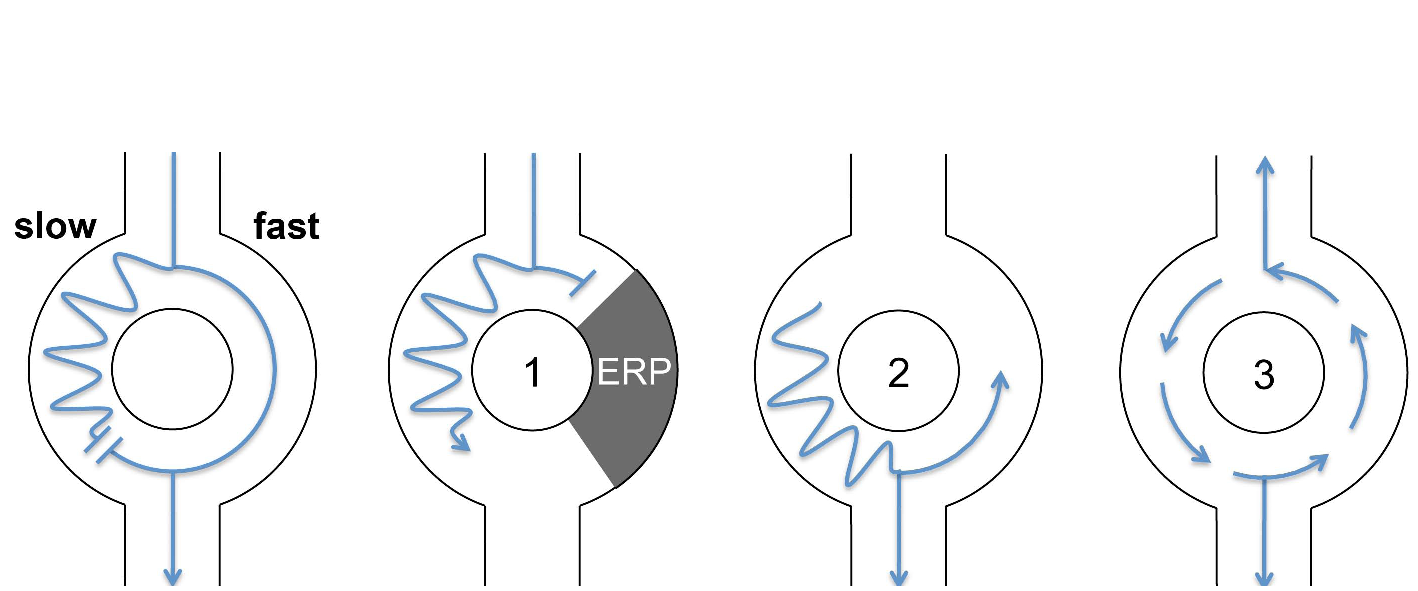
\includegraphics[width=0.6\textwidth]{figs/reentry.pdf}
%%\vspace{-5pt}
%\caption{\small Reentry Circuit}
%%\vspace{-15pt}
%\label{fig:reentry}
%\end{figure}

%\subsubsection{Rule 2: Remove Irrelevant Structures}
The network of node and path automata can be viewed as a graph,with nodes as vertices, paths as edges with conduction delay as weight. After the loops within the topology are removed, the topology of the heart model is in form of tree. Within the network there are certain nodes that are more important in terms of model behaviors, we denote them as \emph{Nodes of Interests}, which include:
\begin{itemize}
\item Nodes with self-activations
\item Nodes which interact with the pacemaker
\end{itemize}
Graph algorithm can be performed on the heart model to identify the core structure. Shortest paths can be calculated among nodes of interests. All the nodes and paths along the shortest paths are regarded as core structure. All the other nodes and paths can be then removed without affecting the behaviors of the model. 
%\todo[inline]{Not true. Teh behavior is affected. Because this is a formal methods conference, so behavior and so on mean very specific things.}
\subsubsection{Rule 3: Removing Unnecessary Non-self-activation Nodes}
The effect of non-self-activation nodes is blocking electrical events with interval shorter than its ERP period. If the self-activation nodes at both ends of a core path have self-activation interval longer than the maximum ERP period of nodes along the core path, the nodes can be removed.

For a core path from a self-activation node $N_1$ to another core node $N_2$, for any structure $P_1-N_n-P_2$ which $N_n$ is a non-self-activation node, if $N_n.ERP_{max}<min(N_1.Rest_{min},N_2.Rest_{min})$, replace $P_1-N_n-P_2$ with $P_3$ so that:
$$P_3.cond_{min}=P_1.cond_{min}+P_2.cond_{min}$$
$$P_3.cond_{max}=P_1.cond_{max}+P_2.cond_{max}$$

\subsection{Rule 4: Merge Parameter Ranges}
\textbf{Physiological intuition}. 
The guards and invariants of node automata define timing periods of the heart, like the Effective Refractory Period (ERP) and Rest period. 
By expanding these periods, we introduce new behavior where a heart may stay in rest for longer, or (self-)activate a node faster, or tissue can conduct current sooner, etc.

\textbf{(Sub)graph(s) to which it applies}.
This rule applies to a set of graphs $G_i$ with the same structure (i.e. isomorphic) but possibly with different parameters: $R(G_1,\ldots,G_n) = G'$.
See Fig.~\ref{fig:HM_abs}.

\textbf{Applicability conditions}.
None.

\textbf{Output (sub)graph $G'$}.
$G'$ has same structure as the $G_i$.
Thus $R$ plays the role of an isomorphism between every $G_i$ and $G'$.
Given an element $x$ of $G'$, we abuse notation by writing $R^{-1}(x') = \{x_1,\dots,x_n\}$ is the set of elements that map to it via $R$.

\textbf{Effect on parameters}
Recall Def.~\ref{def:labeledGraph}
For every automaton $A_{x'} \in \Ac(G')$, and every parameter $\theta^{x'}$ of $A_{x'}$, 
\[\theta_{min}^{x'} = \min(\theta^x_{min})_{x \in R^{-1}(x') }\]
\[\theta_{max}^{x'} = \max(\theta^x_{max})_{x \in R^{-1}(x') }\]

\textbf{Proof of abstraction}.

%\subsection{Rule 5: Merge Self-activation Nodes with Interaction Nodes}
%\todo[inline]{not clear}
The effect of self-activation nodes on the interaction of the pacemaker is triggering sensing events within certain delay. In this rule we merge all the self-activation nodes to their neariest interaction nodes. If there exists multiple self-activation nodes merging to the same interaction node, the parameters of the new model are determined following Rule 3.


\subsection{Rule 6: Replace Blocking With Non-deterministic Conduction}
\textbf{Physiological intuition}. 
Consider the structure $N_1 P_1 N_2 P_2 N-3$ with three nodes and two paths, where $N_2$ is a passive node (i.e. not self-activating).
If $N_2$ blocks an activation signal from $N_1$ to $N_3$, this is equivalent to the paths $P_1$ or $P_2$ not conducting.
In this rule, we replace the structure $P_1 N_2 P_2$ by a path $P$ whose automaton can take a self loop when it receives an activation signal, thus effectively stopping the conduction. 
This is shown in Fig.~\ref{fig:rule5}: the extra transitions are marked {\quattrofont Act\_path\_1?} and {\quattrofont Act\_path\_2?}.
Because the blocking effect of nodes is now incorporated into the paths, we can also modify the node automata of self-activating nodes to the one shown in Fig.~\ref{fig:rule5}, which doesn't have the (now useless) ERP period.

\textbf{Subgraph to which it applies}.
Line graphs with 3 vertices $N_1 P_1 N_2 P_2 N_3$, and self-activating nodes.

\textbf{Applicability conditions}.
$N_2$ is a passive node.

\textbf{Output subgraph}.
A path $P$ whose path automaton is as shown in Fig.~\ref{fig:rule5}.
The self-activating nodes $N$ are replaced by nodes $N'$ with automata shown in Fig.~\ref{fig:rule5}.

\textbf{Effect on parameters}
For the new path, $P.cond_{min}=P_1.cond_{min}+P_2.cond_{min}$ and 
$P.cond_{max}=P_1.cond_{max}+P_2.cond_{max}$
For the new nodes, $N'.Trest_{min}=N.TERP_{min}+N.Trest_{min}$ and 
$N'.Trest_{max}=N.TERP_{max}+N.Trest_{max}$.


\textbf{Proof of abstraction}.

\begin{figure}[!h]
	\centering
	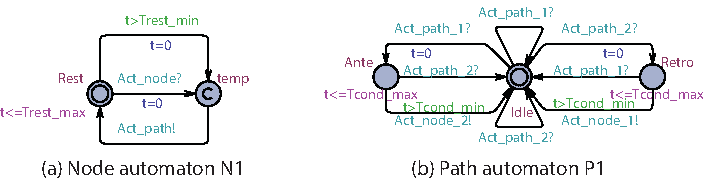
\includegraphics[width=0.9\textwidth]{figs/rule5.pdf}
	%\vspace{-5pt}
	\caption{\small Automata of Rule 5}
	%\vspace{-15pt}
	\label{fig:rule5}
\end{figure}

\subsection{Rule 7: Replace Conductions With Self-activation}
\textbf{Physiological intuition}. 
This rule applies only after Rule 5 has been applied, and sensing nodes have been merged with self-activation nodes.

The effect of a conduction path is to conduct electrical activity generated by a self-activation node to other nodes. 
If we simply allow all self-activation nodes to activate at any time by setting their Rest period to $+\infty$, we can remove all the conduction paths, while preserving the original behavior (where the Rest period was constrained to a finite interval).

\textbf{Subgraph to which it applies}.
The entire graph $G$.

\textbf{Applicability conditions}.
This rule can only be applied after Rule 5 has been applied.

\textbf{Output subraph}.
All edges are deleted: $G' = (V(G), \emptyset)$.

\textbf{Effect on parameters}
For every node automaton $N$ in $G'$, $N.Trest = +\infty$.

\textbf{Proof of abstraction}.

\begin{figure}[!h]
	\centering
	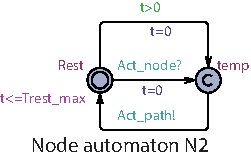
\includegraphics[width=0.3\textwidth]{figs/rule6.pdf}
	%\vspace{-5pt}
	\caption{\small Heart Model Abstractions}
	%\vspace{-15pt}
	\label{fig:rule6}
\end{figure}

\subsection{Heart Model Abstraction Tree}
We first develop a list of concrete heart models corresponding to common heart conditions. 
By systematically applying rules from Section \ref{ruleBasedHeartModelAbstraction} we created an abstraction tree $HM\_tree$ for the heart (\figref{HM_abs}). 
Note that applying rules in different order results different abstraction tree. 
The order used to obtain $HM\_tree$ is based on the domain knowledge that certain heart conditions may have similar behaviors and similar inputs to the pacemaker. 
This systematic grouping maintains the physiological-relevance of the heart model even at higher abstraction levels, and reduce the necessity to resolve ambiguities at lower abstraction levels when model checking certain requirements.
\begin{figure}[!t]
	\centering
	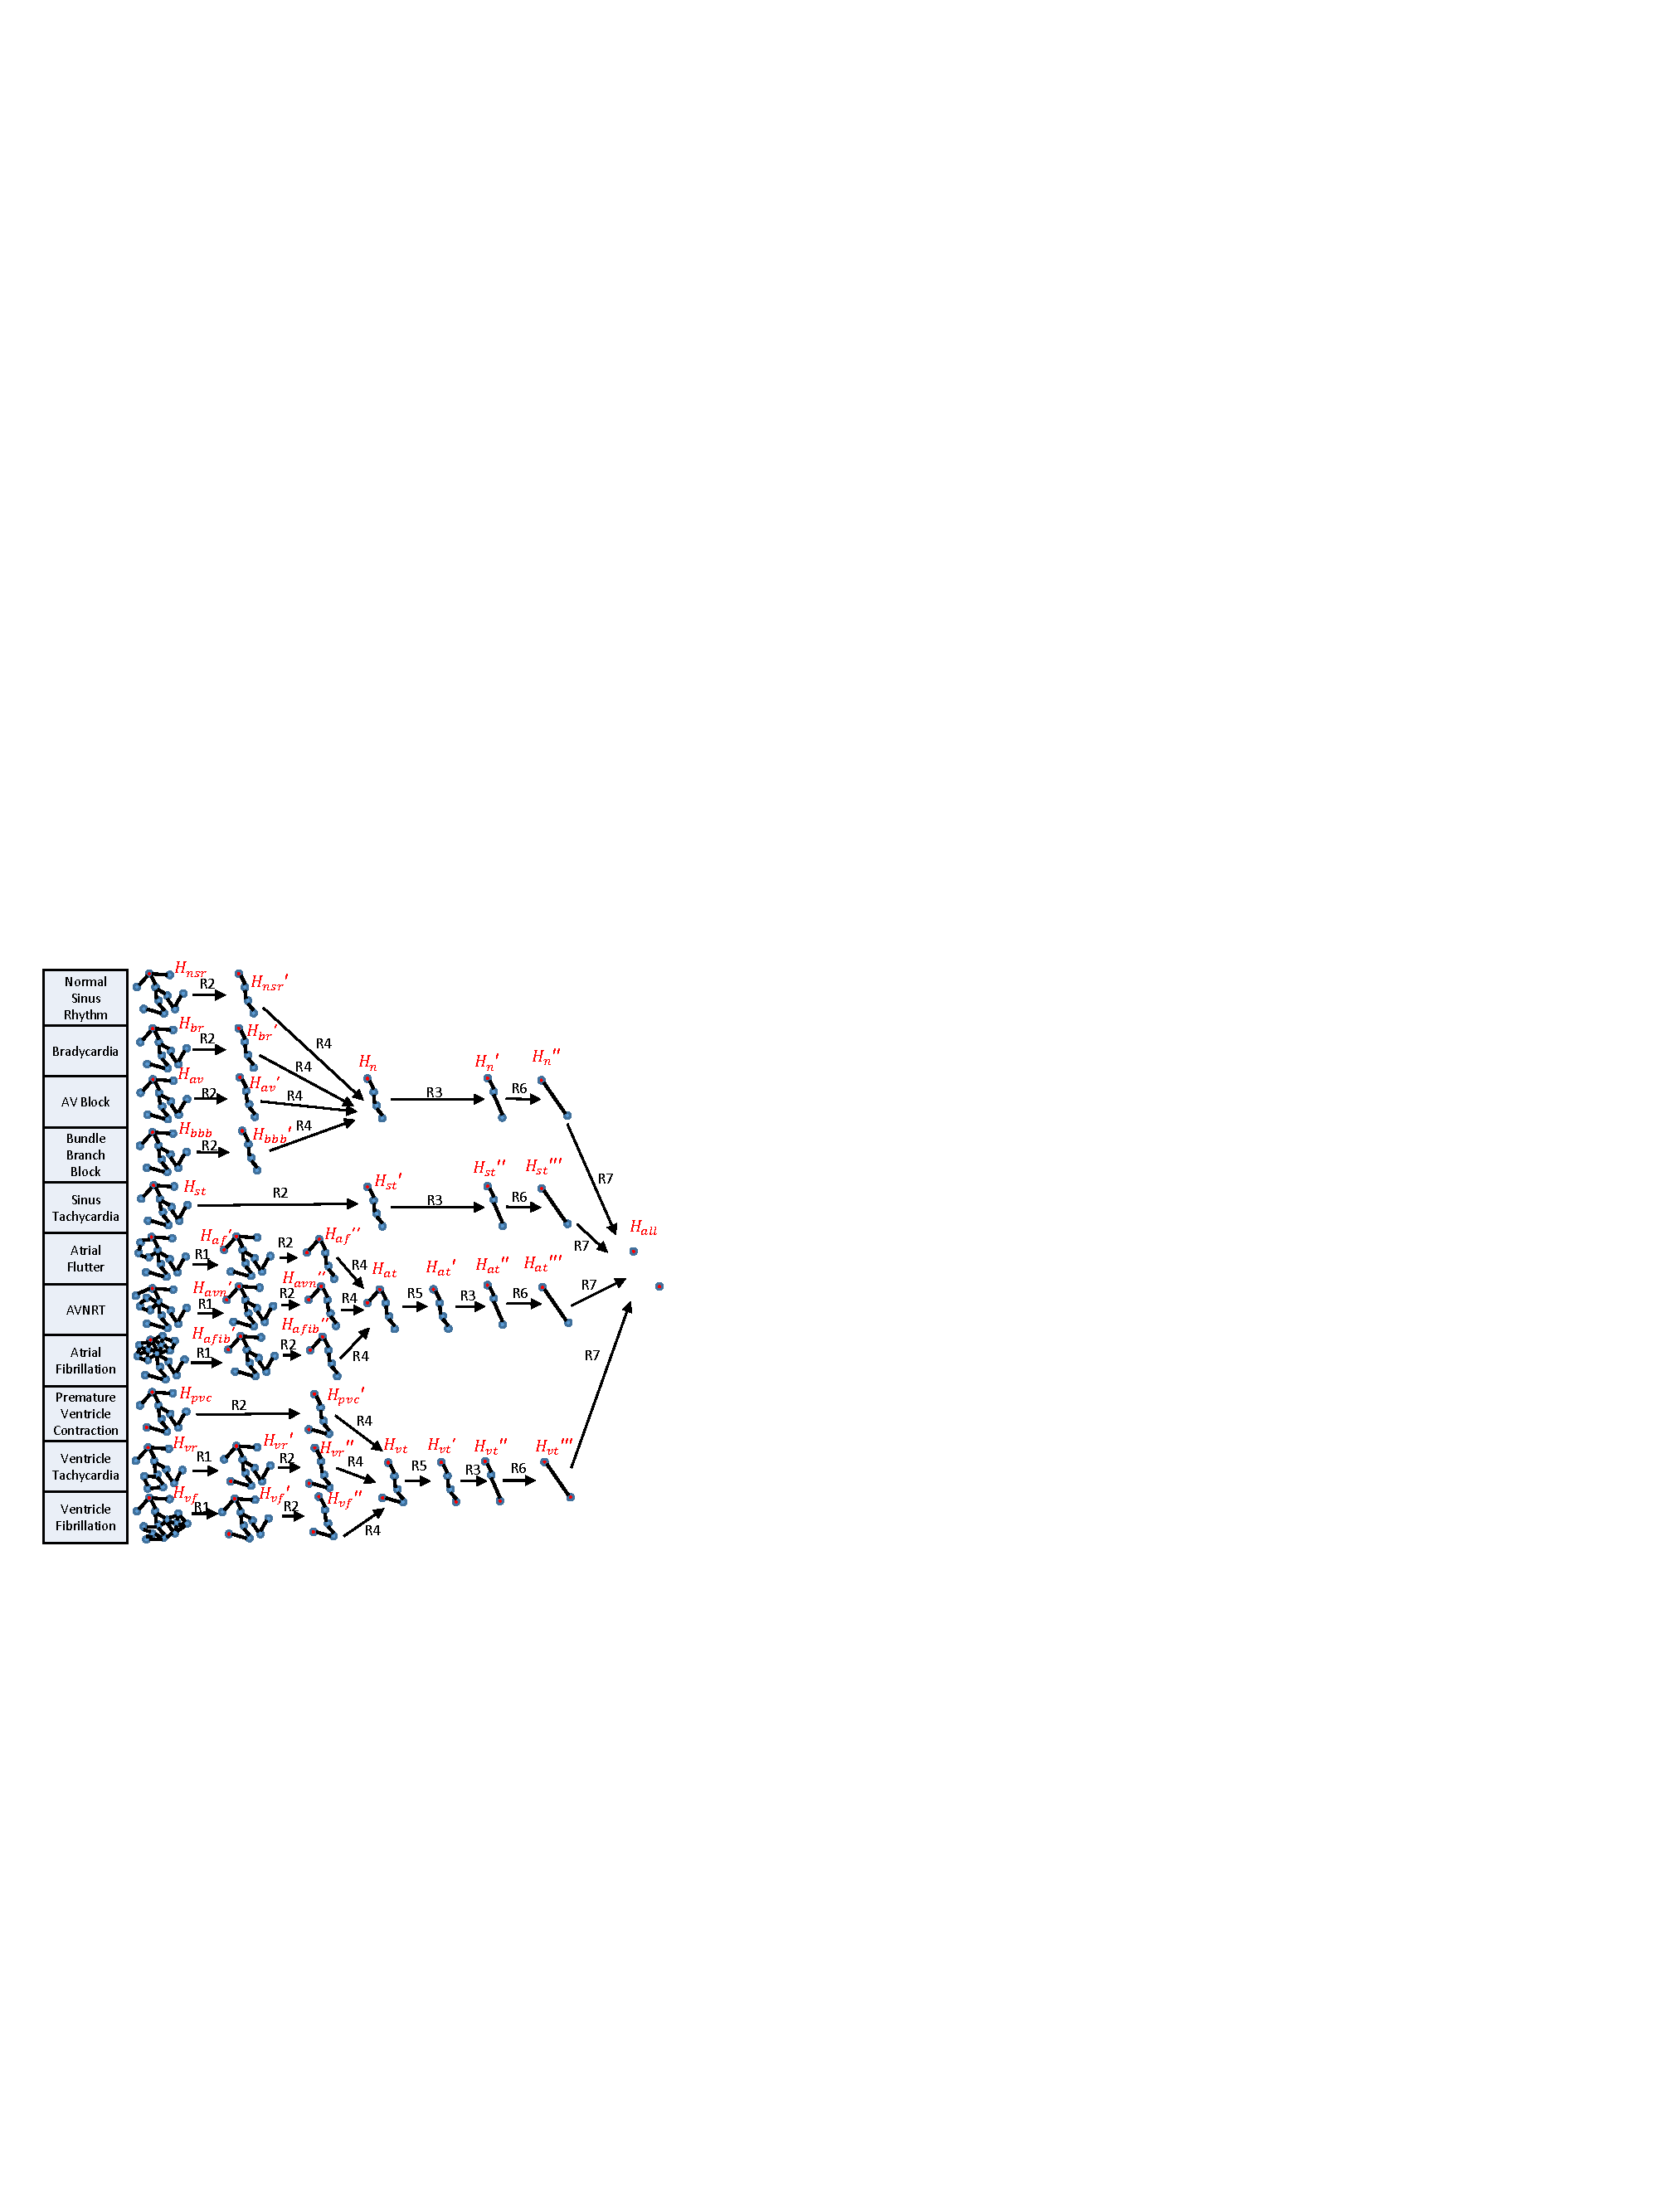
\includegraphics[width=0.9\textwidth]{figs/abs.pdf}
	%\vspace{-5pt}
	\caption{\small Heart Model Abstractions}
	%\vspace{-15pt}
	\label{fig:HM_abs}
\end{figure}

Besides model structure changes, applying abstraction rules also merges the behaviors of the model, which is documented for each abstraction. Here we demonstrate the behavior merging process on a subset of the abstraction tree (\figref{HM_abs}). In $H_{vt}''$, we have self activation behavior $NA.self$ and $NV.self$ for node $NA$ and conduction behavior $NV$,$(NA,AV').cond$ and $(AV',NV).cond$ for path $(NA,AV')$ and $(AV',NV)$. After applying Rule 6 we obtain $H_{vt}''$ with
$$NA'.self=\{NA.self\},NV'.self=\{NV.self\}$$
$$(NA',NV').cond=\{AV'.block,(NA,AV').cond,(AV',NV).cond\}$$
After applying Rule 7 we obtain $H_{all}$ with:
$$NA''.self=\{NA.self,(NA',NV').cond\}$$
$$NV''.self=\{NV.self,(NA',NV').cond\}$$
These information on behavior abstractions are useful to determine whether a model is appropriate for a requirement.
\begin{figure}[!t]
	\centering
	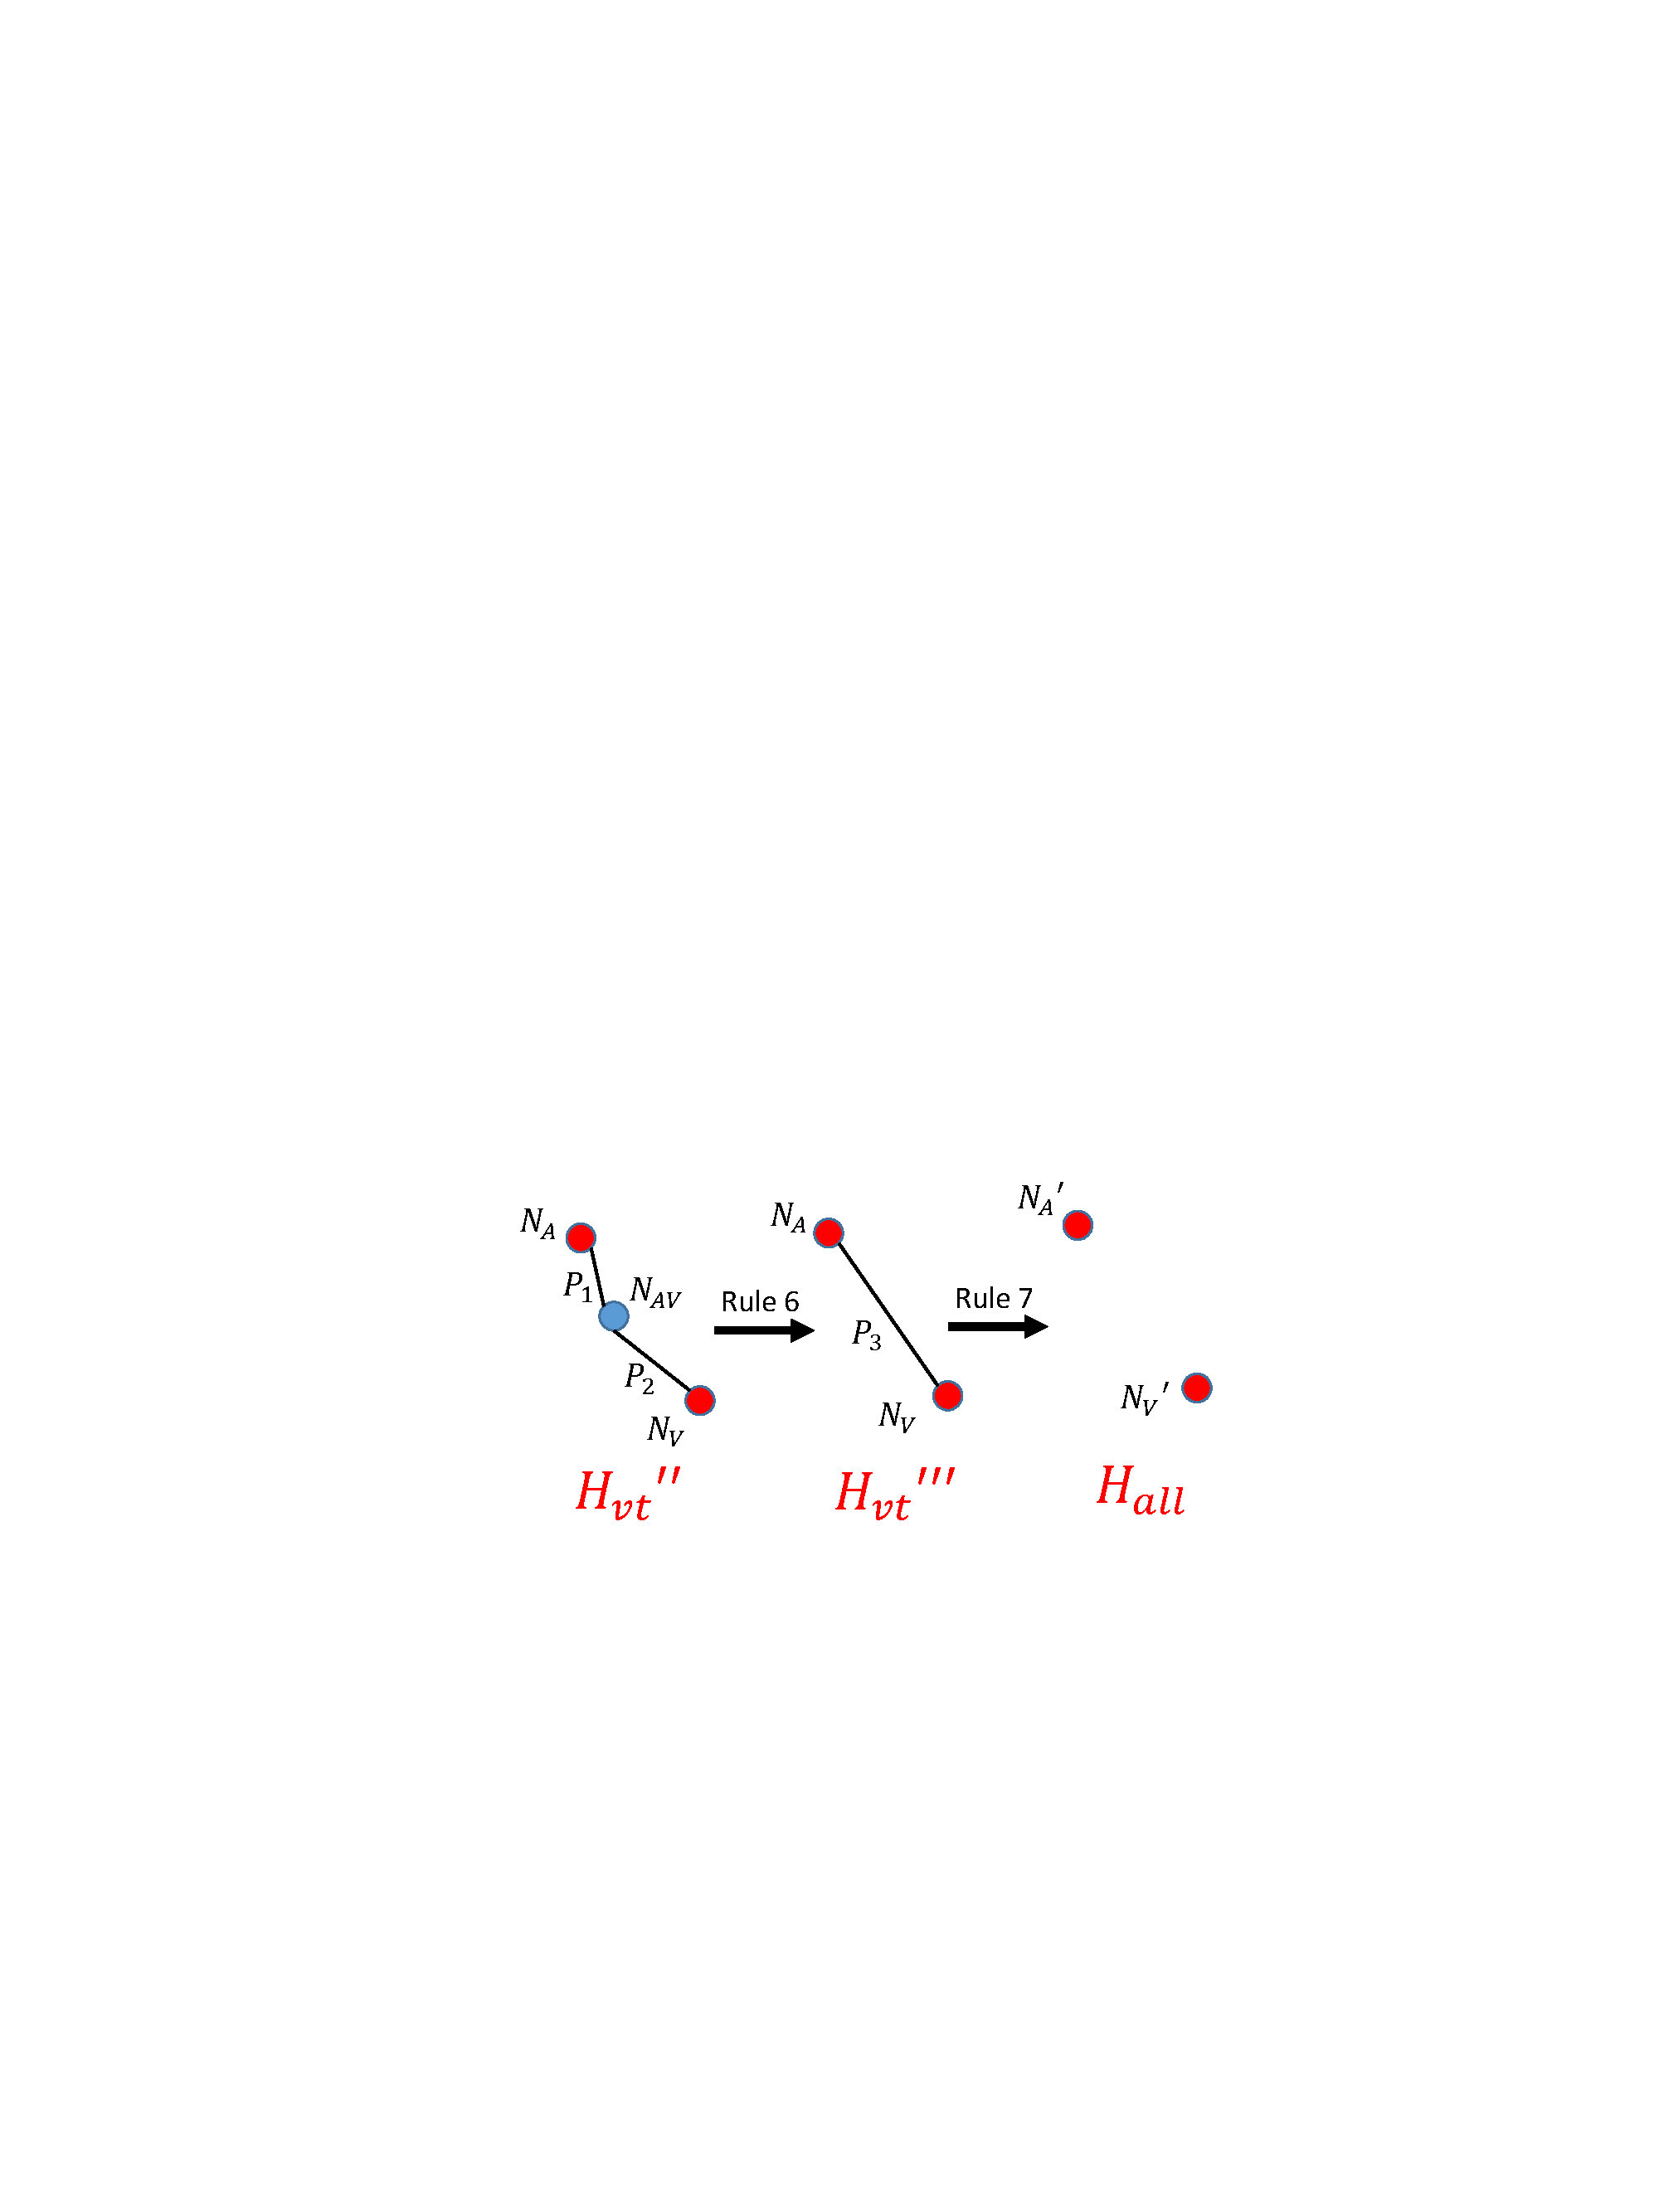
\includegraphics[width=0.5\textwidth]{figs/abs_sim.pdf}
	%\vspace{-5pt}
	\caption{\small Abstraction Example}
	%\vspace{-15pt}
	\label{fig:abs_exam}
\end{figure}
%\subsection{Rule Application Example}
%In this section we demonstrate 
%\todo[inline]{I don't understand what this is...}
%$$NA\_self=\{SA\_self,AVNRT\_self,AF\_self,PAC\_self\}$$
%$$NV\_self=\{PVC\_self,VF\_self,VT\_self\}$$
%$$(NA,AV')\_cond=\{(SA,AV)\_cond\}$$
%$$(AV',NV)\_cond=\{(AV,RBB)\_cond,RBB-RVA\_cond\}$$
%Apply Rule 6:
%$$NA'\_self=\{NA\_self\}$$
%$$NV'\_self=\{NV\_self\}$$
%$$(NA',NV')\_cond=\{AV'\_block,(NA,AV')\_cond,(AV',NV)\_cond\}$$
%Apply Rule 7:
%$$NA''\_self=\{NA'\_self,(NA',NV')\_cond\}$$
%$$NV''\_self=\{NV'\_self,(NA',NV')\_cond\}$$
%\begin{figure}[!t]
%\centering
%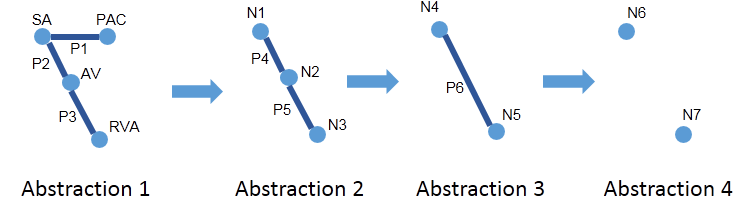
\includegraphics[width=0.9\textwidth]{figs/abs.png}
%%\vspace{-5pt}
%\caption{\small Heart Model Abstractions}
%%\vspace{-15pt}
%\label{fig:abs_exam}
%\end{figure}

\section{Model checking with the abstraction tree}
\label{modelCheckingwAbstTree}


	\begin{enumerate}
		\item Measure of abstractness; define 'appropriate for the requirement'
		\item Search procedure
		\item What happens if a counter-example is found
		\item Elaborate example
		\end{enumerate}
\section{Closed-loop Model Checking Using the Abstraction Tree}
After the abstraction tree is built, it can be used for closed-loop model checking. The next question is how to navigate through the abstraction tree so that the most appropriate model(s) are selected for different requirements, and provide the most concrete counter-examples, possibly under multiple physiological conditions, for the physicians to determine the validity of the counter-examples. %\cite{uppaal}
\subsection{Select Initial Abstraction(s) Appropriate For the Requirement}
%Physiological requirements are in general conditional in the sense that they require conditions to hold under certain open-loop physiological constraints. These constraints map to parameters for certain transitions of the physiological models, which may be merged during the abstraction process.
For a requirement $Req$ and its auxiliary 
The most abstract model in the abstraction tree is built to cover the input space to the device as much as possible, thus it may not have enough details to constrain the behaviors of the model according to the constraints in the requirement. Thus the first step of closed-loop model checking is to select the most abstract models which are appropriate for the requirement. A model $M$ is appropriate for a requirement $Req$ if the environment transitions mentioned in the requirement, denoted as $EnvT(Req)$, is a subset of the environment transitions associated with the model $EnvT(M$). The following algorithm finds the most abstract heart models in the abstraction tree $HM\_tree$ that are appropriate for a requirement $Req$.
\begin{Verbatim}
Algorithm 1
function [HM]=eligible(HM_tree,Req)
BM = root of HM_tree
while (BM is not empty)
 For every model M in BM
  If (Var(Req)\cap Var(Mon) is a subset of Var(M))
   Remove M from BM
   save M in HM
  else
   add children of M in BM
  endif
 endfor
endwhile
Return HM
\end{Verbatim}
%BM = all models in HM_tree with all Prop(Req)
%For all M in BM
 %while (in the parent of M no behavior in Prop(Req) is abstracted with other behaviors)
	 %M = parent of M
 %endwhile
 %save M in HM
 %endfor
\subsection{Obtaining Concrete Counter-examples Under Corresponding Physiological Conditions}
One challenge for modeling physiological environment of medical devices is the large variety of physiological conditions that the devices may encounter. %It is impossible to exhaustively model the conditions with concrete physiological models. 
The set of concrete models (the leave nodes in the abstraction tree) only represent a subset of all possible physiological conditions, thus model checking the device on all of the concrete models is not enough to guarantee the satisfaction of the requirement. By applying physiological abstraction rules, additional physiological-relevant behaviors are incorporated into the abstract models by over-approximation, providing more coverage. 
However, if model checking on an abstract model returns a counter-example, if is difficult to determine whether the counter-example is a valid execution. Due to the incomplete nature of the set of concrete models, if the counter-example cannot be concretized on all the concrete models, it does not mean it is invalid. Therefore it is up to the physician to decide whether a counter-example is valid or not. The algorithm below explore the abstraction tree during model checking and provide the physician the most concrete counter-example(s), if there exists any. 
\begin{Verbatim}
Algorithm 2
Input: system model PM, abstraction tree for environment HM_tree, requirement Req
Output: Counter examples CE and corresponding model refinements
[HM]=eligible(HM_tree,Req);
Mc= HM;
 while (Mc is not empty)
  For all M in Mc
   [satisfied,CE]=ModelChecking(M,PM,Req);
	 Remove M from Mc
	 If satisfied==0
	  add the children of M to Mc
		cache CE
	else
		save CE from the parent model
	endif
 endfor
endwhile
Return all saved CEs and their corresponding models
\end{Verbatim}

\section{Case Study: Closed-loop Model Checking of a Dual Chamber Pacemaker}
\subsection{Pacemaker Model}
\begin{figure}[!t]
		\centering
		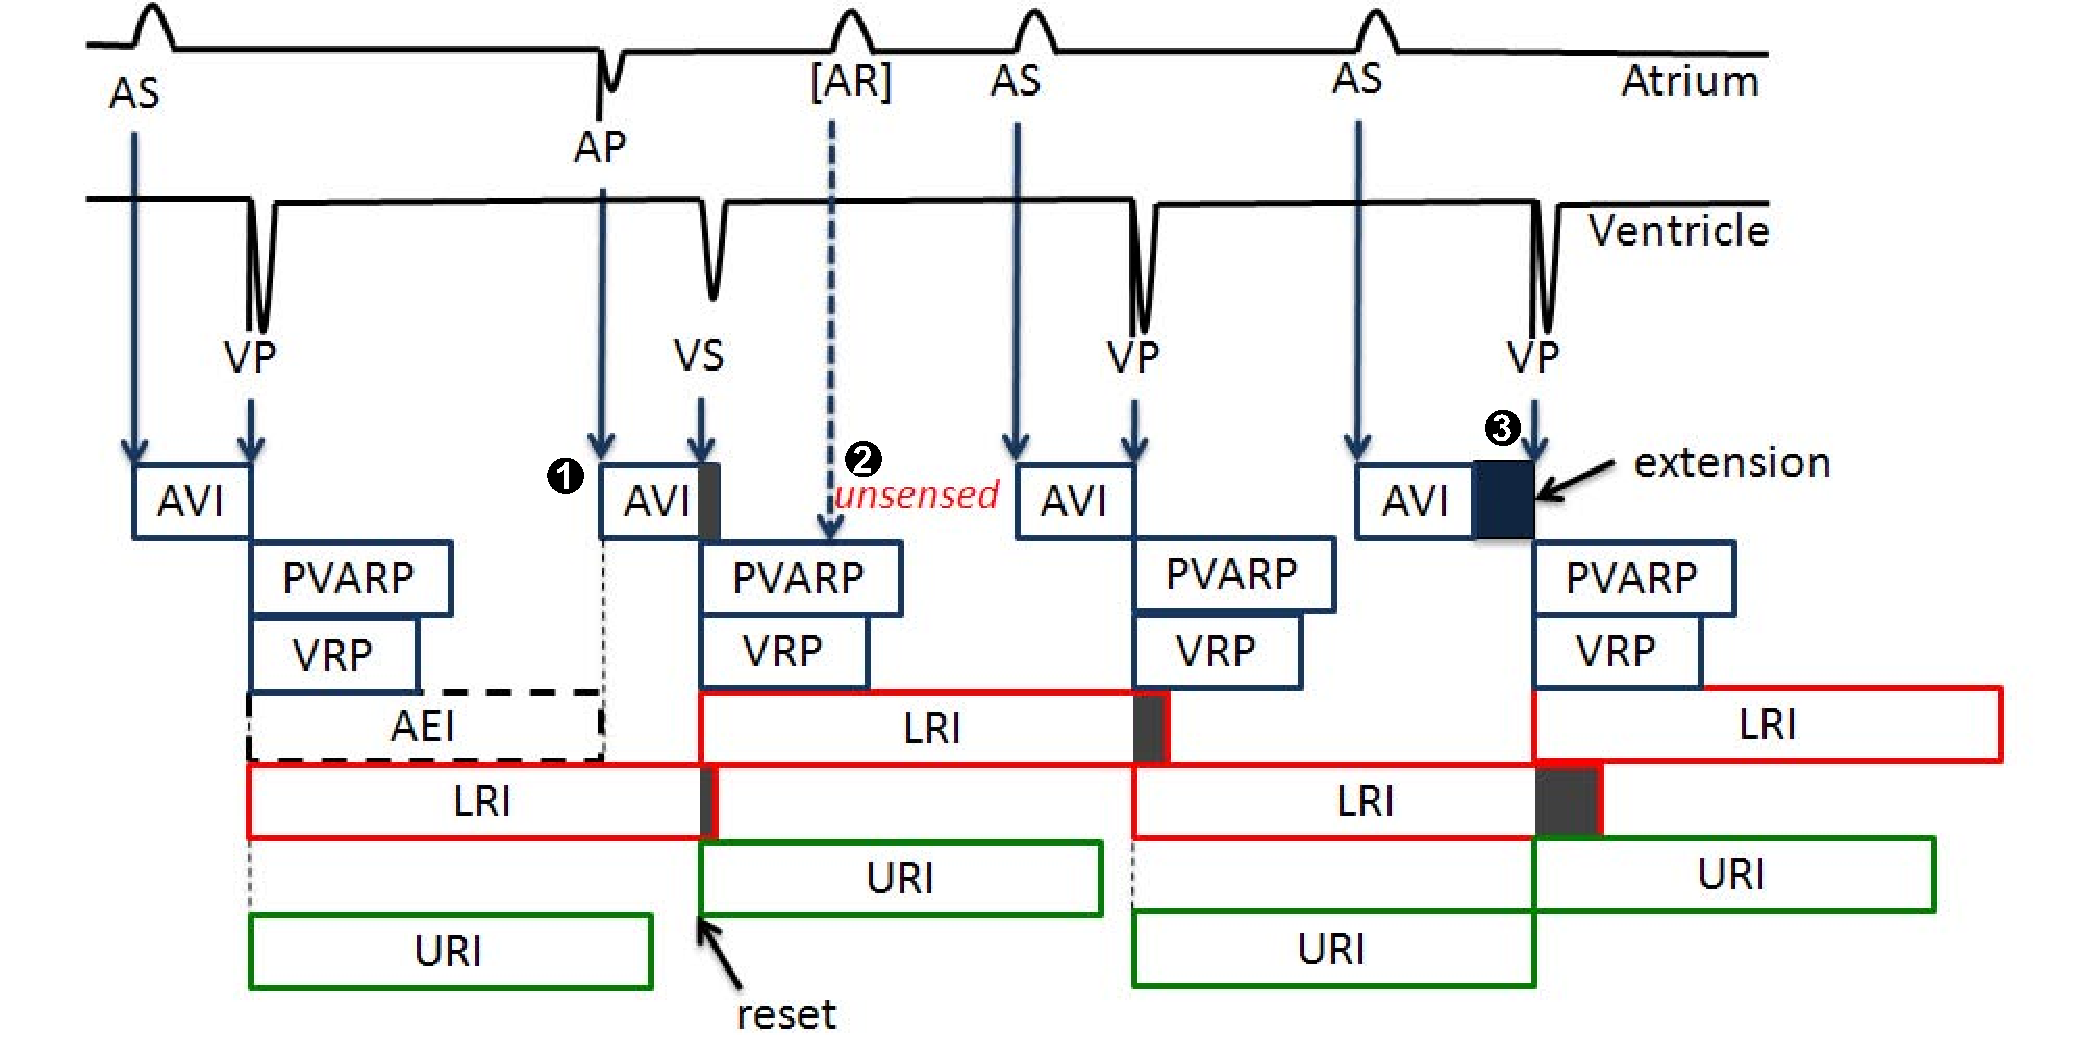
\includegraphics[width=0.5\textwidth]{figs/PM_timers.pdf}
		%\vspace{-5pt}
		\caption{\small Heart Model Abstractions}
		  %\vspace{-15pt}
		\label{fig:PM_timers}
\end{figure}

\subsection{Requirement Encoding}
Physiological requirements can be automatically mapped to model behaviors and parameters. In general, a requirement has \emph{pre-conditions} under which the requirement should hold. The pre-conditions are open-loop physiological conditions which are in terms of constraints on model behaviors. The \emph{post-conditions} are closed-loop behaviors that the device should achieve. The requirement below is designed to prevent the pacemaker from pacing too fast.
\begin{itemize}
	\item Pre-condition: Atrial self-activation rate (60bpm - 200bpm)
    \item Post-condition: Intervals between ventricular paces should be no shorter than 500ms
\end{itemize}

With behavior mapping and a monitor (\figref{monitor}), the requirement can be translated to:
$$Req1: NA.self.min=300 \&\& NA.self.max=1000 \Rightarrow not M.Err$$
The environment behavior specified in $Req1$ is $EnvB(Req1)=NA.self$.
\subsection{Choosing Appropriate Heart Model For the Requirement}
To verify the closed-loop system with pacemaker model $PM$ and heart model abstraction tree $HM\_tree$ (\figref{abs_exam}) against requirement $Req1$, we start by searching for the most abstract appropriate models from the abstraction tree. We call the function specified in Algorithm 1: $[HM]=eligible(HM\_tree,Req1)$. At the root level heart model $H_{all}$, $NA.self$ is abstracted with $(NA',NV').cond$. As the result, $H_{all}$ is not appropriate for $Req1$. $NA.self$ is not abstracted with other behaviors in the children of $H_{all}$: $H_n'',H_{at}'''',H_{vt}'''$, thus these 3 heart models are outputted as the most abstract appropriate models for $Req1$.
\subsection{Providing Meaningful Counter-examples to the Physicians}
After we choose the appropriate models for $Req1$, we have: 
$$HM=\{H_n'',H_{at}'''',H_{vt}'''\}$$
Then we run Algorithm 2. By model checking on all 3 initial models in UPPAAL we have: 
$$[1,[]]=ModelChecking(H_n'',PM,Req1)$$
 $$[0,CE_1]=ModelChecking(H_{at}'''',PM,Req1)$$
$$[0,CE_2]=ModelChecking(H_{vt}''',PM,Req1)$$
The algorithm keeps going down the abstraction tree, and at certain intermediate step we have:
 $$[0,CE_a]=ModelChecking(H_{st}',PM,Req1)$$
  $$[0,CE_b]=ModelChecking(H_{pvc}',PM,Req1)$$
	$$[0,CE_c]=ModelChecking(H_{at},PM,Req1)$$
 $$[1,[]]=ModelChecking(H_{vr}'',PM,Req1)$$
 $$[1,[]]=ModelChecking(H_{vf}'',PM,Req1)$$

\begin{figure}[!t]
		\centering
		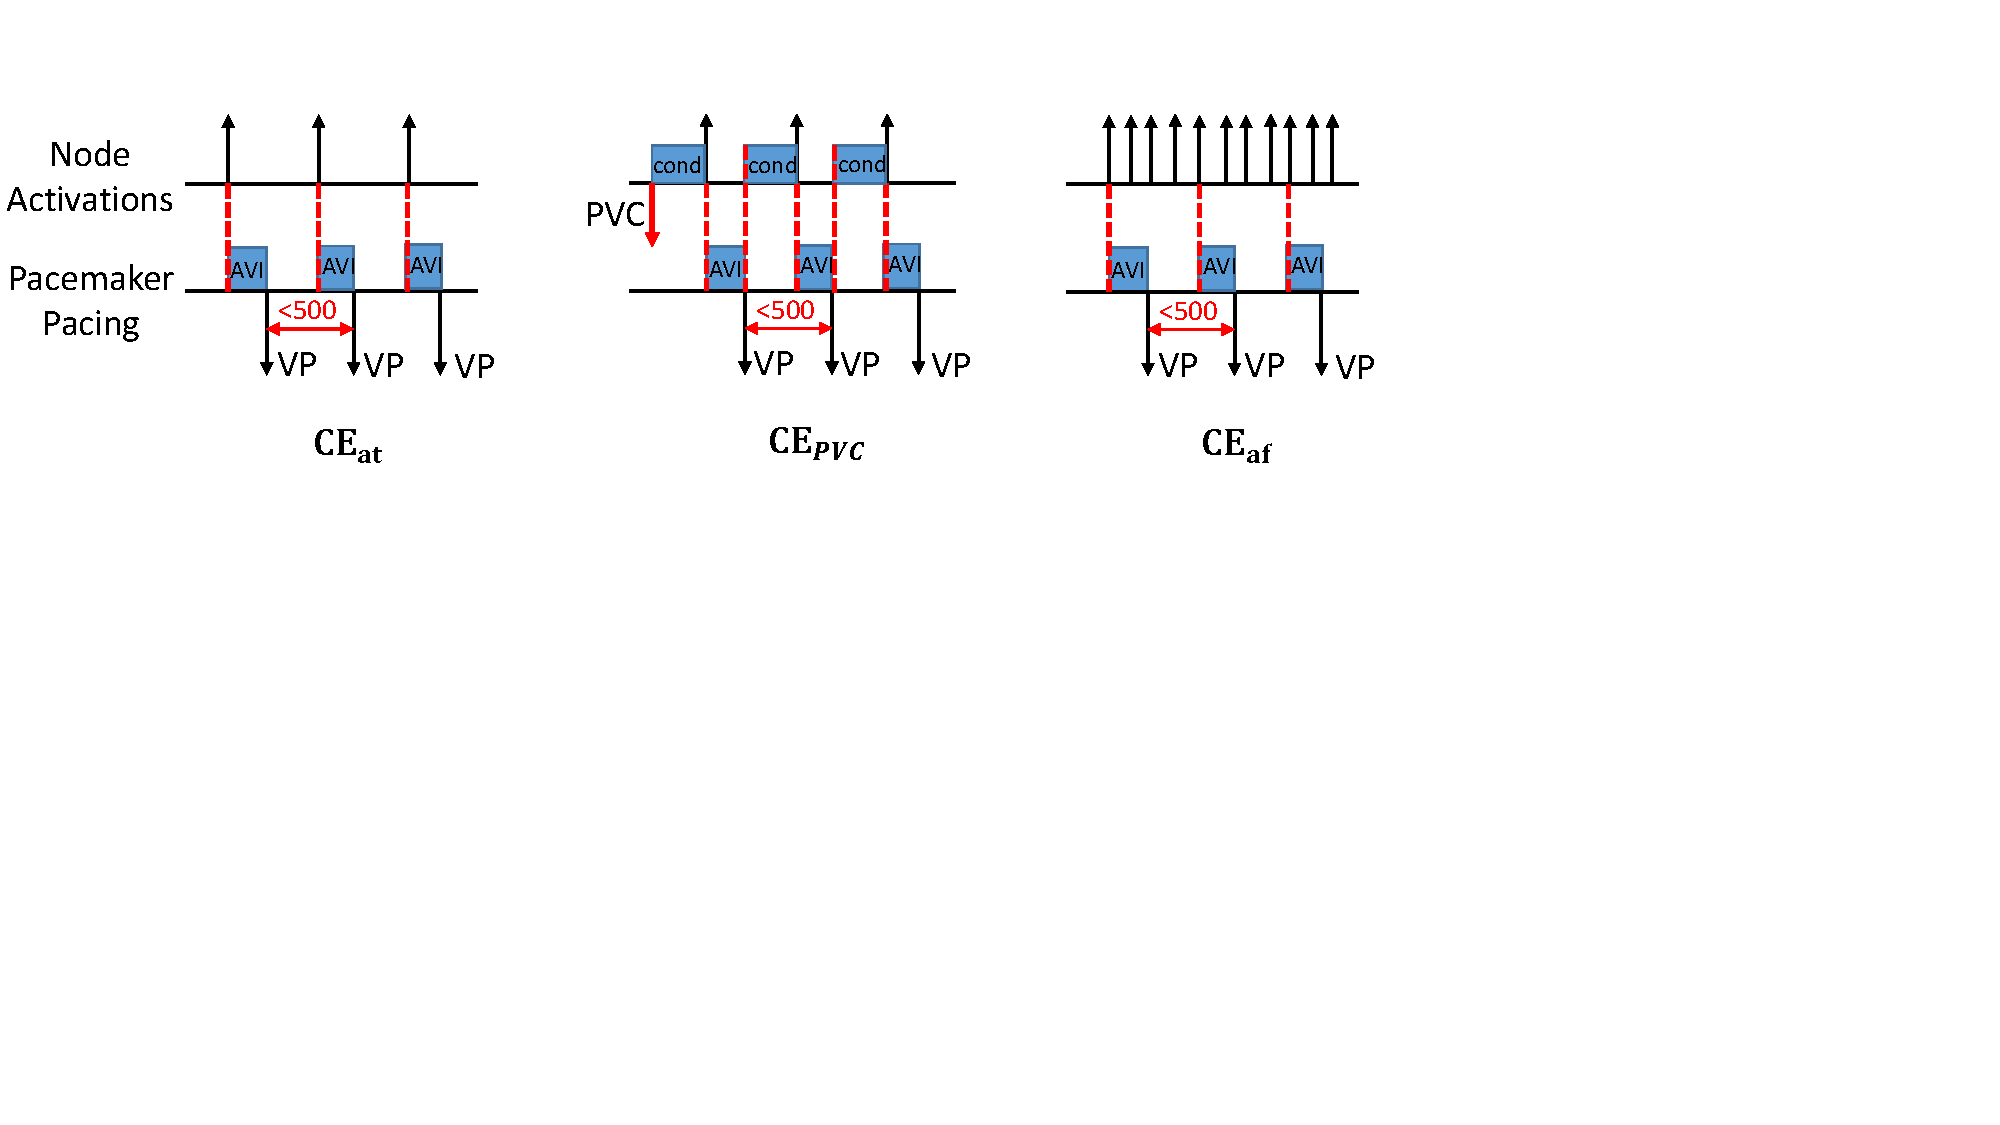
\includegraphics[width=0.9\textwidth]{figs/case.pdf}
		%\vspace{-5pt}
		\caption{\small Counter-examples}
		  %\vspace{-15pt}
		\label{fig:CE}
\end{figure}
The counter-examples from more refined models provide more detailed mechanism of the requirement violations, and distinguish the physiological conditions that can trigger the violations. It is much easier for the physician to determine the validity of the counter-example. The counter-examples from the example above are illustrated in \figref{CE}. $CE_a$ corresponds to fast intrinsic heart rate thus is a safe execution of the pacemaker. $CE_b$ corresponds to a scenario called Endless Loop Tachycardia during which the pacemaker and the heart forms a conduction loop that increases the heart rate inappropriately. In $CE_c$ the pacemaker extends fast atrial rate to more dangerous fast ventricular rate, which is referred to as Atrial Tachycardia Response of a pacemaker. Both $CE_b$ and $CE_c$ are inappropriate executions of the pacemaker .$CE_a$ and $CE_b$ can have the same input-output executions on the pacemaker side and can only be differentiated on the heart model side. After the physician examines the counter-example the programmer can work on debugging.
%$NA\_self$ is in $H_3$, we go one level up, in $H_4$ the behavior is not merged with any other parameters. In $H_5$ $NA\_self$ is merged with  $NA'-NV'.cond$ so $H_4$ is returned as the appropriate heart model for R1. In \cite{STTT13} we used $H_4$ to verify the correctness of the ELT termination algorithm. With a basic DDD pacemaker we have $H_4 || P_{DDD}\models R1$. The counter-example returned is exactly the ELT behavior. Then we implement the ELT termination algorithm and we have  $H_4 || P_{ELT}\not\models R1$, meaning ELT has been successfully terminated, and only the ELT is terminated. 
%
%\subsection{Inappropriate Model Refinements}
%If we follow the traditional CEGAR framework and verify the property using $H_5$, an abstract counter-example would return, which is shown in %\figref{C_amiguity}. However the counter-example correspond
 






\section{Conclusions and future research}
\label{conclusions}


\newpage
\section{\textcolor{red}{Case 2: Resolving Validity Ambiguities Using Model Refinement}}
\label{resolvingValidityAmbiguities}
\subsection{Atrial Tachycardia and Mode-switch}
\subsection{Requirement Encoding}
\begin{itemize}
	\item Pre-condition: Atrial Tachycardia, vent  ricular rate normal
    \item Post-condition: No increase in ventricular rate
\end{itemize}
\subsection{Identify potential ambiguities}

\begin{itemize}
	\item Utilizing the assumptions made during abstraction Rule 3
    \item Replacing ERP with non-deterministic conduction can potentially increase the number of activations
    \item Two possible refined executions
    
\begin{itemize}
	\item Valid 
    \item Invalid
\end{itemize}
    \item Undo Rule 3
    \item Refine to $H_2$
\end{itemize}

%\section{Bullet Points}
\label{bulletPoints}
\subsection{Specification vs. Requirement}
\begin{itemize}
	\item Requirements are specified in terms of conditions of the \textbf{environment} before and after the system is deployed
    \item Specifications are specified in terms of how the system responds to an input sequence from the environment
    \item Traditional verification focus on specification of the system
    \item Verifying specification only need to consider the input-output sequence of the system, which does not require knowledge of the environment
    \item The result only provide guarantees for the correctness of the system. But what about the correctness of the specifications themselves?
   
    \item In CPS especially, the focus should be more on whether specifications satisfy requirements, which is also an important aspect in requirement engineering.
    
    \begin{itemize}
        
        \item Requirements are specified by domain experts and requires deep domain knowledge 
        \item Traceability between requirements and specifications are currently maintained by mostly documentation
        \item Verifying requirements requires closed-loop verification
    \end{itemize}
\end{itemize}
\subsection{Closed-loop Verification}
\begin{itemize}
    \item For medical devices, closed-loop verification is currently done in terms of clinical trials, which has following problems:
    \begin{itemize}
      \item The cost of clinical trials are high
      \item Due to the cost, the scale of the clinical trials cannot be large, thus affecting patient generality and the effectiveness of the trials.
      \item It is the last step of the design process thus discovering a bug at this stage is very costly to fix.
	\end{itemize}
	\item Model-based design can potentially enable closed-loop verification at early design stage
    %\item The biggest challenge for model-based design is to develop validated models, for both the system and the environment
\end{itemize}
    
\subsection{Closed-loop Verification using Model Checking}
\begin{itemize}
	\item Model checking explore the state space of the closed-loop model and identify potential safety violations
    \item Model checking is usually performed on abstract models.  
    \item Obtaining exact abstractions are computationally hard
    \item Over-approximation is often used during the abstraction step
        \begin{itemize}
        	\item \textbf{Pros: }Simple abstraction procedure 
            \item \textbf{Cons: }Introducing spurious counter-examples
        \end{itemize}
    \item Over-approximation usually introduces non-determinism, which can achieve:
    \begin{itemize}
        	\item \textbf{Simplisity: }Non-determinism can replace complex dynamics which are not useful during the analysis
            \item \textbf{Generality: }Sometimes the model should be able to capture the behaviors of different variations of the entity under modeling, which can be achieved using non-determinism.
        \end{itemize}
    \item Over-appproximation is complete for $ACTL^*$, meaning if a property in $ACTL^*$ holds in the abstract model, it will also hold in the refined model
\end{itemize}



\subsection{Model Abstraction Level Management}
\begin{itemize}
	\item The model should not only be abstract enough to achieve generality and simplisity, but also need to contain enough information to express the \emph{interesting} behaviors of the entity being modeled.
    \item Abstraction may introduce ambiguity due to the information loss
    \item Ambiguities should be eliminated in the following levels:
\end{itemize}
\textcolor{red}{
\begin{enumerate}
	\item \textbf{A1: Input-output Relation: }Executions that generates different outputs should be distinguishible in the abstract model
    \item \textbf{A2: Requirement Compatibility: }If two executions in the refined model are made indistinguishible in the abstract model, either both satisfy the requirement or both violate the requirement
    \item \textbf{A3: Execution Validity: }One execution which violates a requirement needs to be valid in the refined model to be considered as a counter-example.
\end{enumerate}}
These 3 ambiguities are increasing difficult to eliminate.
\subsubsection{Counter-Example-Guided Abstraction and Refinement (CEGAR)}
CEGAR is a framework to manage the model complexity during model checking of system specifications. It starts with a concrete representation of the system (code usually).
\begin{enumerate}
	\item Obtain the initial abstraction of the system
    \item Ensure the initial abstraction is compatible with the specification in checking (Satisfying A2)
    \item Model checking the model against the specification
    \begin{enumerate}
        \item If no counter-example returned, the specification is satisfied
        \item If a counter-example returns, validate the counter-example on the concrete system
        \begin{enumerate}
            \item If the counter-example is valid, a bug has been found
            \item If the counter-example is invalid, identify the \emph{deadend state} and \emph{error state}
        \end{enumerate}
    \end{enumerate}
    \item Refine the model to seperate deadend state and error state (Satisfying A3)
    \item Go back to step 3.
\end{enumerate}
CEGAR works very well for managing abstraction level of system model during specification verification.

\subsection{System Model vs. Environment Model}
The system and the environment have very different characteristics, thus requires different approaches during modeling.
\begin{itemize}
	\item Non-determinism
    \begin{itemize}
    	\item It is normally desired that a system is deterministic, thus there is only one desired output sequence given an input sequence. As the result, the non-determinism of a system model is usually minimal.
        \item In medical device industry especially, a device is designed to treat large variations of patients. The behaviors of the same patient cannot be modeled with a deterministic model. As the result, the environment model needs to generalize the variations using non-determinism. 
    \end{itemize}
    \item Observability
        \begin{itemize}
        	\item It is considerably easy to observe the state of the system. For the software part of the system, we can even achieve full observability
            \item On the other hand, it is very hard to (non-invasively, in-vivo) put sensors in the environment to achieve the same granularity of observability.
        \end{itemize}
    \item Internal mechanism 
    \begin{itemize}
    	\item Since the system is built by human, we have near full knowledge of the internal mechanism, allowing us to build a detailed and accurate model or representation (i.e. code) of the system.
        \item Largely due to the limited observability, we have very partial knowledge about the environment. Even these knowledge are not easily accessible to the system developers.
    \end{itemize}
\end{itemize} 

\subsection{Incapability of CEGAR for Environment Model Refinement}
\begin{itemize}
	\item CEGAR is not directly applicable for requirement verification and abstraction level management of the environment model
	\item Step 3 and 4 in the CEGAR framework cannot be done for environment model  
    \begin{itemize}
    	\item A counter-example is spurious only if it does not exist in any of the environment conditions, which is impossible to check due to the non-determinism and the large variety of the environment model.
        
        \item Without identifying the deadend state and error state in the model, there is no heuristic to guide model refinement
    \end{itemize}
    \item\textcolor{red}{Cannot solve the ambiguity of the environment condition specified in the requirement. (need formulation)}
\end{itemize}


\subsection{Bridging the knowledge gap}
In model-based design of Cyber-Physical Systems, there are two parties involved who have distinct expertise in their fields:
\begin{itemize}
	\item \textbf{Domain experts} processes \textbf{domain knowledge}, which is how the environment works, through years of training and experiences. In the medical devices domain, the domain experts are physicians. The role of the domain experts are:
        \begin{itemize}
        	\item Specify requirements in terms of environment conditions before and after the system is deployed into the environment
            \item Validate an execution trace if the execution trace is fully or partially from a model simulation.
            \item Evaluate (not validate) environment conditions in terms of closed-loop executions
        \end{itemize}
    
    \item \textbf{System developers} are the ones who develop the system to control the environment. System developers generally have deep knowledge of the system under development, but with limited knowledge of the environment. The role of the system developers are:
        \begin{itemize}
        	\item Propose system specifications to satisfy environmental requirements
            \item Verify the system against system specifications
        \end{itemize}
\end{itemize}
The two parties need to work interactively together, however it is clear that there are knowledge gaps between the two parties. There are certain tasks that require knowledge in both domains that neither parties can perform on their own.
\begin{itemize}
	\item Environmental model construction
    \item Environmental model abstraction
    \item Environmental model refinement
\end{itemize}

A third party, tool developer, can help in this regard.
\begin{itemize}
	\item \textbf{Behaviors} are used to describe environment executions, even conditions
    \item Encode the domain knowledge into different behaviors of the environment
    
    \begin{itemize}
        \item \textbf{Requirements} by linking environmental conditions with series of high-level behaviors
        \item \textbf{Environment models} by assigning behaviors to the models
        \item \textbf{Abstraction rules} by documenting how behaviors are merged or ignored during each abstraction step.
    \end{itemize}
    \item For domain experts, their requirements are automatically converted into model-checking-friendly form.
    \item For system developers, given the requirement, the tool should be able to provide the (almost) most abstract environment model without any ambiguities mentioned in Section 1.4.
    \item As the result, both parties can focus on their expert domain.
    \item Without the help of counter-examples, this approach cannot fully eliminate spurious counter-examples
\end{itemize}
 


% \subsubsection{Domain Knowledge During Abstraction Level Management}
% Although CEGAR is not directly applicable to the environment model, the knowledge of how the environment works can be used during the abstraction level management. 

% The domain knowledge contains:


% \begin{itemize}
%     \item Distinguish environment conditions specified in the requirement
% 	\item Using domain knowledge a counter-example can be regarded as spurious, although sometimes not 100\%. (Physicians can say that some conditions are very unlikely to happen, but not impossible)
% \end{itemize}

% \begin{itemize}
    
   
%     \item The system and the environment have very different characteristics, thus requires different approaches during modeling.
%     \begin{itemize}
%         \item We have full or near-full knowledge of the system:
%         \begin{itemize}
%             \item The system has one single deterministic implementation or the non-determinism is minimal
%             \item The internal mechanism of the system is 
%             \item Observability of the system is maximal
%         \end{itemize}
%      	\item
%     \end{itemize}
%     \item \textbf{Model validation}: Given the same input sequence, the model should be able to produce equivalent or close enough output as the corresponding entity being modeled.
            
%     \item System modeling
% \end{itemize}

%Medical device is a typical Cyber-Physical System and ensuring the safety and efficacy of the device requires closed-loop verification. Currently closed-loop verifications of medical devices are performed in the form of clinical trials in which the devices are tested on the patients. Using clinical trials as closed-loop verification has several problems:

% In \cite{VHM_proc} we addressed the problems above by proposing a model-based design framework to enable closed-loop verification earlier in the design stage. The increased confidence in safety and efficacy of the device can potentially reduce the scale of the clinical trials, thus reduce cost.

% In model-based design for Cyber-Physical Systems, both the system and its environment are abstracted as models. One of the widely used abstraction technique is \emph{over-approximation}. The benefits of over-approximation are:
% \begin{itemize}
% 	\item Reducing verification complexity by removing details of the system or the environment.
% 	\item Generalizing different system/environment conditions
% \end{itemize}
% However, there are inevitable infomation losses during over-approximation. The biggest challenge for model-based design is obtaining correct abstraction levels of the models and managing the information loss during the abstraction steps. 

% Although over-approximation 




\bibliographystyle{abbrv}
\bibliography{bibliography}
\end{document}